% ============================================================================
%  main.tex
%  西南科技大学本科生毕业论文（设计）
%  题目：虚拟问诊系统设计与实现
%  作者：柏彪  学号：5120223930  专业：大数据2203
%  编译命令：xelatex main → bibtex main → xelatex main → xelatex main
% ============================================================================
\documentclass[zihao=-4, UTF8, openany, oneside, a4paper]{ctexbook}

% ---------- 自定义格式宏包 ----------
\usepackage{swust-thesis}

% ---------- 参考文献：GB/T 7714-2015 ----------
\usepackage[backend=biber, style=gb7714-2015, gbnamefmt=lowercase, sorting=none]{biblatex}
\addbibresource{refs.bib}
\defbibenvironment{bibliography}
  {\list
     {}
     {\setlength{\leftmargin}{0pt}%
      \setlength{\labelwidth}{0pt}%
      \setlength{\labelsep}{0pt}%
      \setlength{\itemindent}{0pt}%
      \setlength{\itemsep}{\bibitemsep}%
      \setlength{\parsep}{\bibparsep}}}
  {\endlist}
  {\item\printtext[labelnumberwidth]{\printfield{labelprefix}\printfield{labelnumber}}\hspace{1em}}

% ---------- 封面元信息 ----------
\swusttitle{虚拟问诊系统设计与实现}
\swusttitleen{Design and Implementation of a Virtual Consultation System}
\swustauthor{柏\hspace{2em}彪}
\swustno{5120223930}
\swustmajor{数据科学与大数据技术}
\swustadvisor{XXX\hspace{1em}副教授}
\swustcollege{计算机科学与技术学院}
\swustdirection{人工智能与软件工程}
\swustdate{二〇二六年六月}

\begin{document}

% ============================================================================
% 前置部分：摘要、目录
% 页码：罗马数字 I, II, III, ...
% ============================================================================
\frontmatter
\pagenumbering{Roman}

% ---- 中文摘要 ----
% ============================================================================
% 中文摘要
% 写作要点：
%   1. 第一段（背景与意义，约130字）：医学问诊实训痛点 + 大模型机遇
%   2. 第二段（系统设计与实现，约180字）：前后端分离架构 + 三角色 +
%      四模块 + 关键基础设施
%   3. 第三段（创新点与结果，约180字）：Agent 编排层 + RAG + Memory +
%      临床工具 + 结构化评分 + 部署测试
%   4. 关键词 6 个，与英文严格对应
%   5. 总字数控制在 500 字左右
% ============================================================================

\begin{abstractzh}

\noindent{\heiti\zihao{-4} 摘要：}问诊训练需要病例、标准化病人与教师反馈共同支撑，但在高校日常教学中，真实病例不易反复开放，标准化病人成本较高，教师也很难逐轮跟进每名学生的训练过程。大语言模型为虚拟病人提供了新的实现途径，不过直接依赖提示词容易出现角色越界、检查结果编造和反馈笼统等问题。基于此，本文围绕医学问诊实训设计并实现虚拟问诊系统，重点解决训练过程可交互、病例事实可约束、训练结果可复盘的问题。

系统采用前后端分离架构。前端基于 Vue 3、TypeScript 和 Element Plus 构建，后端使用 Spring Boot 3.3.6、Java 17 与 MyBatis-Plus 实现；MySQL 保存用户、病例和训练记录，Redis 维护验证码、登录锁定和会话上下文，MinIO 存储医学影像与附件，Docker Compose 用于部署。系统面向学生、教师、管理员三类用户，提供 AI 问诊训练、病例库管理、学习分析和系统管控等功能，并集成 JWT 认证、RBAC 权限控制、ECharts 可视化和 SSE 流式响应。

在 AI 实现上，系统将单一提示词调用拆分为 PatientAgent、DiagnosisAgent 和 FeedbackAgent 三类角色，由 AgentRouter 按训练阶段选择调用对象；关键词检索式 RAG 用于补充医学知识，Redis 滑动窗口保存最近多轮对话，临床工具优先从病例数据返回体格检查、辅助检查和影像结果，避免模型自行生成客观数值。训练结束后，系统以结构化 JSON 输出问诊、诊断、治疗、沟通等维度评分，并在解析失败时使用规则兜底。系统已完成云端部署和功能、性能、安全测试，能够支持医学问诊训练的基本闭环。

\keywordszh{医学教育；虚拟问诊；大语言模型；AI Agent；检索增强生成；前后端分离}

\end{abstractzh}


% ---- 英文摘要 ----
% ============================================================================
% 英文摘要
% 写作要点：
%   1. 与中文摘要严格三段对应
%   2. 全文使用 Times New Roman 12pt（小四）
%   3. Keywords 使用英文分号分隔，与中文关键词逐项对应
% ============================================================================

\begin{abstracten}

\noindent{\fontspec{Times New Roman}\bfseries\zihao{-4} Abstract: }Medical inquiry training depends on clinical cases, standardized patients and timely teacher feedback. In routine university teaching, however, these resources are not always available for repeated practice. Large language models make virtual patients more feasible, but a prompt-only solution may easily cross role boundaries, fabricate examination results, or provide vague feedback. This thesis therefore designs and implements a virtual consultation system for medical inquiry training, with an emphasis on interactive practice, controllable case facts and reviewable training results.

The system follows a front-end / back-end separated architecture. The front end is developed with Vue 3, TypeScript and Element Plus, while the back end uses Spring Boot 3.3.6, Java 17 and MyBatis-Plus. MySQL stores users, cases and training records; Redis keeps verification codes, login locks and dialogue context; MinIO manages medical images and attachments; Docker Compose is used for deployment. For students, teachers and administrators, the system provides AI consultation training, case-library management, learning analytics and system administration, together with JWT authentication, RBAC authorization, ECharts visualization and SSE streaming.

For the AI workflow, the system separates a single prompt into three roles: PatientAgent, DiagnosisAgent and FeedbackAgent. AgentRouter selects the proper role according to the training stage. A keyword-based RAG module supplies medical knowledge, Redis memory keeps recent dialogue turns, and clinical tools return physical examination, auxiliary examination and imaging results directly from case data instead of allowing the model to invent objective findings. After training, the system outputs structured JSON scores for inquiry, diagnosis, treatment and communication, with rule-based fallback when parsing fails. Deployment and functional, performance and security tests show that the system can support a complete medical inquiry training loop.

\keywordsen{Medical Education; Virtual Consultation; Large Language Model; AI Agent; RAG; Front-end / Back-end Separation}

\end{abstracten}


% ---- 目录 ----
\cleardoublepage
\pagestyle{frontmatter}
\tableofcontents

% ============================================================================
% 主体部分：正文
% 页码：阿拉伯数字 1, 2, 3, ...
% ============================================================================
\mainmatter
\pagenumbering{arabic}
\setcounter{page}{1}
\pagestyle{thesisplain}

% ============================================================================
% 第 1 章 绪论
% 预估页数：3-4 页
% 写作总要点：
%   - 写 "为什么做这件事"，不写技术细节
%   - 围绕 "医学问诊实训痛点 + LLM 与 Agent 时代机遇" 展开
%   - 国内外研究现状必须有真实文献引用（首次引用同时加脚注）
% ============================================================================
\chapter{绪论}

% ----------------------------------------------------------------------------
\section{研究背景与意义}
% 写作要点：
%   1. 第一段（背景）：医学教育数字化趋势 + 临床实习资源紧张 + 标准化病人
%      （SP）成本高、规范化训练机会有限
%   2. 第二段（机遇）：以 ChatGPT、GPT-4、通义千问为代表的 LLM 在医学领域
%      取得突破 \cite{singhal2023clinicalknowledge,kung2023chatgpt}
%   3. 第三段（意义）：构建一个面向医学院校的 AI 模拟诊疗系统，可解决：
%      (1) 病例数量与多样性受限；(2) 教师批量指导效率低；(3) 学情难量化
%   4. 提一句"本课题的创新点是引入多 Agent 协同与 RAG，超越简单的 LLM 套壳"

医学问诊（Medical Inquiry）连接医患沟通、临床思维与诊疗决策，是医学生临床技能训练中的基础环节。国家关于医学教育创新发展和教育信息化建设的文件均提出，要推动信息技术进入人才培养过程\cite{gov2020mededu,moe2018eduinfo}。但在实际教学中，问诊训练往往依赖课堂讲授、临床见习和标准化病人（Standardized Patient，SP）演练\cite{zhao2012sp}，资源供给并不稳定：真实病例受隐私和伦理约束，难以反复用于教学；标准化病人的招募、培训和维护成本较高；教师逐一复盘学生问诊过程也需要大量时间。随着医学生规模扩大，这些问题会直接影响课后练习次数和反馈质量。

近几年，以 GPT-4、通义千问等为代表的大语言模型（Large Language Model，LLM）在医学问答、考试评测和临床推理任务中表现出较强的语言理解能力。国内已有研究讨论 ChatGPT 对医学教育的影响\cite{qu2023chatgpt}，中文医疗大模型综述也强调，中文医疗语境下仍需专用数据集、评测体系和安全控制\cite{ji2024chinesemedllm}。HuatuoGPT\cite{zhang2023huatuogpt}、Qwen\cite{bai2023qwen}等模型的出现，使高校在中文场景中构建虚拟病人和训练反馈系统的门槛降低。国外研究中，Singhal 等\cite{singhal2023clinicalknowledge}和 Kung 等\cite{kung2023chatgpt}也从医学知识问答和考试角度验证了大模型的潜力。

不过，把通用大模型直接放进问诊训练并不可靠。单靠提示词约束时，模型有时会一边扮演患者，一边主动提示诊断或治疗方案；遇到血常规、影像描述等客观结果时，也可能生成病例中不存在的数值。问诊结束后的评价如果仍停留在自然语言建议，教师也难以形成可统计的学情数据。针对这些问题，本课题在通义千问模型之上加入多 Agent 协同、RAG、临床工具自动注入和结构化评分机制，设计并实现面向医学院校的虚拟问诊系统，使系统既能用于学生反复训练，也能为教师批改和教学分析提供数据基础。

% ----------------------------------------------------------------------------
\section{国内外研究现状}

% ----------------------------------------------------------------------------
\subsection{医学教育数字化研究现状}
% 写作要点：
%   - 国外：Harvard Medical School 的 OSCE 数字化、SP 训练系统
%   - 国内：人卫慕课、丁香医生模拟训练、各医学院校建设的虚拟仿真平台
%   - 局限：以静态脚本为主，缺乏交互能动性

医学教育数字化的探索可以追溯到 20 世纪 90 年代以计算机辅助教学为代表的电子病例库与多媒体教学系统。进入 21 世纪以来，随着 Web 技术与多媒体内容生产能力的发展，国外医学院校逐步建立了以临床综合考核（Objective Structured Clinical Examination，OSCE）数字化、虚拟病人（Virtual Patient）与高仿真模拟人（high-fidelity simulator）为代表的实训体系，部分研究还将虚拟病人与游戏化交互机制相结合，以增强学生的沉浸感和决策训练效果。在国内，随着"互联网 + 教育"政策的推进，人民卫生出版社相继建设了医学慕课和电子题库，多家医学院校依托国家级虚拟仿真实验教学项目建设了系统化的虚拟仿真实训平台，覆盖问诊、查体、急救等典型临床场景\cite{liu2021virtualsim}。

总体来看，传统数字化方案多采用预设脚本、决策树问答或知识点填空。它们的优势是流程可控、内容安全，但交互空间有限，学生很难像真实问诊那样自由追问，系统也难以根据薄弱点给出个性化反馈。因此，问诊实训需要从“内容搬到线上”进一步转向“训练过程可交互、可分析”。

% ----------------------------------------------------------------------------
\subsection{大语言模型在医学教育中的应用}
% 写作要点：
%   - Med-PaLM 在 USMLE 上达到 67\% \cite{singhal2023clinicalknowledge}
%   - ChatGPT 通过执业医师考试 \cite{kung2023chatgpt}
%   - 通义千问、ChatGLM-Med、HuatuoGPT 等中文医疗大模型
%   - 局限：直接 prompt LLM 容易"出戏"、给出诊断答案、缺乏教学层级

近三年来，大语言模型在医学教育领域的应用研究迅速增长。国内研究已经从教学模式、能力培养、风险防控等角度讨论了 ChatGPT 类生成式人工智能对医学教育的影响\cite{qu2023chatgpt}；中文医疗大模型研究则进一步围绕医疗咨询、医学影像、心理健康等任务梳理了中文医疗大模型的发展脉络与评测挑战\cite{ji2024chinesemedllm}。在模型实践层面，HuatuoGPT\cite{zhang2023huatuogpt}通过医学问答数据和医生真实数据增强模型的医疗咨询能力，Qwen\cite{bai2023qwen}系列模型则在大规模中英双语语料和指令对齐数据上进行预训练，提供了通用与医学场景兼具的开放接口。国外研究中，Singhal 等\cite{singhal2023clinicalknowledge}和 Kung 等\cite{kung2023chatgpt}也分别从临床知识编码和医学考试评测角度验证了大语言模型辅助医学教育与临床培训的潜力。

这些研究说明，大语言模型具备成为“虚拟病人”或“辅助带教工具”的基础能力。但已有工作更多停留在问答评测层面，对“问诊—检查—诊断—治疗—反馈”这一完整训练链路考虑不足。仅靠提示词也难以长期稳定地控制患者角色、客观检查结果和多轮记忆。要让系统进入常态化教学场景，还需要在模型之上增加工程化的角色分工、知识约束和评价闭环。

% ----------------------------------------------------------------------------
\subsection{AI Agent 与多智能体协作研究现状}
% 写作要点：
%   - ReAct 框架：推理 + 行动 \cite{yao2023react}
%   - Toolformer：让 LLM 学会调用工具 \cite{schick2023toolformer}
%   - LLM 自主 Agent 综述 \cite{wang2024llmagent}
%   - 多 Agent 协作（MetaGPT、AutoGen 等）在领域应用的兴起
%   - 论证：多 Agent + RAG + 工具调用 是当前 AI 应用工程的最佳实践

将大语言模型扩展为具有记忆、规划和工具使用能力的 AI Agent，是近年大模型落地应用的重要方向。Yao 等\cite{yao2023react}提出的 ReAct 框架把推理与行动交替组织起来，使模型可以在多步任务中调用外部工具；Schick 等\cite{schick2023toolformer}进一步讨论了模型学习工具调用的可能性。Lewis 等\cite{lewis2020rag}提出的 RAG 则通过外部知识检索约束生成内容，缓解幻觉和知识过时问题。这些研究为“提示词 + 检索 + 工具调用”的工程方案提供了基础。

在多智能体协作方向，AutoGen\cite{wu2023autogen}和 MetaGPT\cite{hong2024metagpt}都强调通过角色分工与对话协议完成复杂任务；Wang 等\cite{wang2024llmagent}也指出，医疗、教育等领域会出现更多专用 Agent。本课题借鉴这一思路，把标准化病人扮演、诊断评估和治疗反馈拆成不同 Agent，再由路由器按训练阶段调度，以适应医学问诊实训的教学边界。

% ----------------------------------------------------------------------------
\section{研究目标与主要工作}
% 写作要点：
%   - 研究目标：3 条简洁陈述
%       (1) 构建一套面向医学问诊实训的多角色完整 Web 系统
%       (2) 提出并实现"多 Agent + RAG + 临床工具 + 结构化评分"的医疗
%           AI 模拟诊疗框架
%       (3) 完成系统部署与功能验证
%   - 主要工作：分点列出 5--6 项

本课题的研究目标可以概括为以下三点：

第一，面向医学院校问诊实训需求，设计并实现一套覆盖学生、教师、管理员三类角色的完整 Web 化模拟诊疗系统，提供 AI 问诊训练、病例库管理、学习分析与系统管控等核心功能。

第二，在通用大语言模型之上，构建包含 Agent 编排、知识检索、会话记忆、临床工具与结构化评分的医疗 AI 模拟诊疗框架，提升问诊训练的可控性、客观性与教学反馈质量。

第三，完成系统的容器化部署与测试，检查功能流程、接口响应、安全控制和 AI Agent 效果。

围绕上述研究目标，本文的主要工作包括：

（1）需求分析与总体架构设计。梳理医学问诊实训的业务流程，提炼三类用户的核心需求，给出基于前后端分离与多 Agent 协同的整体架构、数据库 ER 模型与接口规范。

（2）多 Agent 路由的对话引擎实现。抽象 PatientAgent、DiagnosisAgent、FeedbackAgent 三类 Agent 角色，由 AgentRouter 在不同训练阶段动态选择，避免在问诊中出现角色混淆与答案泄露。

（3）轻量化 RAG、滑动窗口 Memory 与临床工具自动注入机制实现。将医学知识、对话历史与客观检查结果以工程化方式注入提示词，规避大模型在客观医学事实上的幻觉风险。

（4）多维结构化评分与规则兜底实现。以 JSON Schema 约束模型输出，给出问诊、诊断、治疗、沟通四个维度的可视化分析与改进建议，并在模型返回异常时通过规则兜底保障评分服务可用。

（5）端到端工程实现与部署测试。基于 Vue 3 与 Spring Boot 完成全栈实现，通过 Docker Compose 完成容器化部署，并从功能、性能、安全维度进行测试与验证。

% ----------------------------------------------------------------------------
\section{论文组织结构}
% 写作要点：
%   - 用一段过渡 + 编号列表说明 8 章内容
%   - 强调第 5 章为核心创新章

本论文围绕“虚拟问诊系统设计与实现”展开，全文共分为八章，按照"问题背景—相关技术—需求分析—架构设计—核心实现—模块详解—测试部署—总结展望"的逻辑层层推进。各章主要内容如下：

第 1 章 绪论。介绍课题的研究背景与意义，综述国内外在医学教育数字化、大语言模型医学应用与 AI Agent 三个方向的研究现状，并明确本文的研究目标、主要工作与组织结构。

第 2 章 相关技术概述。介绍系统涉及的关键技术，包括 Vue 3 前端框架、Spring Boot 后端框架、阿里百炼大语言模型平台、AI Agent 与多智能体协作、检索增强生成、Function Calling 工具调用、MySQL/Redis/MinIO 等数据基础设施以及 Docker 容器化部署。

第 3 章 系统需求分析。从业务、功能与非功能需求等角度分析系统需求，给出三类用户的用例图与典型用例规约。

第 4 章 系统总体设计。阐述系统的整体架构、功能模块划分、数据库 ER 模型、接口设计、RBAC 权限模型与安全架构，为后续的详细实现奠定基础。

第 5 章 AI Agent 核心技术实现。作为本论文的核心创新章节，重点呈现多 Agent 路由、RAG 知识检索、Redis 滑动窗口会话记忆、临床工具自动注入、结构化评分以及 SSE 流式响应等关键模块的设计原理与代码实现。

第 6 章 系统功能模块详细实现。详细介绍学生端、教师端、管理员端及公共模块的关键页面、交互流程与代码实现，覆盖 AI 问诊训练、病例管理、批改工作台、学习分析等业务场景。

第 7 章 系统测试与部署。给出功能、性能、安全与 AI Agent 效果验证的测试方案与结果，并描述系统基于 Docker Compose 的容器化部署过程与运行效果。

第 8 章 总结与展望。对全文工作进行总结，凝练创新点，分析现有不足并给出后续研究方向。

% ============================================================================
% 第 2 章 相关技术概述
% 预估页数：3-4 页
% 写作总要点：
%   - 介绍系统所用的关键技术，每项 200-400 字
%   - 重点是为后续章节（特别是 Agent 章节）做理论铺垫
%   - 不要写成技术说明书，要点出"为何选用 + 在本系统中的作用"
% ============================================================================
\chapter{相关技术概述}

% ----------------------------------------------------------------------------
\section{前端开发技术}

\subsection{Vue 3 与 Composition API}
% 写作要点：
%   - 渐进式框架、响应式系统的优势
%   - Composition API 相对 Options API 在大型项目的逻辑复用优势
%   - 引用 Vue 官方文档 \cite{vuejs2024}

Vue.js 是渐进式 JavaScript 前端框架，适合以组件方式组织中后台页面\cite{vuejs2024}。本系统采用 Vue 3.4.21，其基于 Proxy 的响应式机制更适合处理训练页中不断变化的对话列表、计时状态和表单数据。相比 Options API，Composition API 可以把同一业务关注点集中到一个逻辑单元中，例如将 Agent 状态、SSE 对话流、训练提交和病例信息拆成独立复合函数，避免大型页面的状态散落在多个选项中。系统同时使用 Vue Router、Pinia 和 Vite 完成路由、状态管理与开发构建。

\subsection{Element Plus 与 ECharts}
% 写作要点：
%   - Element Plus 提供企业级 UI 组件
%   - ECharts 用于雷达图（能力评估）、折线图（成绩趋势）、柱状图（知识点掌握）
%   - 引用 \cite{li2018echarts}

Element Plus 是面向 Vue 3 的 UI 组件库，提供表格、表单、对话框、上传和菜单等常用组件。本系统的学生端、教师端和管理员端均基于 Element Plus 2.6.3 构建，并通过 CSS 变量区分不同角色的主题色，减少重复页面开发。

ECharts 用于系统中的学情可视化\cite{echarts2024}。学生端使用雷达图展示问诊、诊断、治疗和沟通四个维度，使用折线图呈现训练成绩变化；教师端则通过柱状图和饼图观察班级知识点错误分布。相比直接展示表格，图表更利于学生复盘和教师发现共性问题。

% ----------------------------------------------------------------------------
\section{后端开发技术}

\subsection{Spring Boot 与 Spring Security}
% 写作要点：
%   - 约定优于配置，自动装配
%   - Spring Security 提供过滤器链、认证授权
%   - 本系统采用 Spring Boot 3.3.6 + Java 17

Spring Boot 在 Spring Framework 基础上提供自动装配和约定式配置，能减少重复工程代码\cite{springboot2024}。本系统采用 Spring Boot 3.3.6 和 Java 17，主要用于提供 REST 接口、SSE 流式对话接口以及与数据库、缓存、对象存储的集成。其 WebFlux 组件被用于调用外部大模型服务，便于处理较长时间的 AI 响应。

Spring Security 负责身份认证和权限控制。本系统在过滤器链中加入 JWT 认证过滤器，从 HTTP 头中读取 Token、验证签名并写入认证上下文；登录、验证码、文件预览等少数路径开放访问，其余接口默认需要认证。该设计能够满足前后端分离系统的基本安全边界。

\subsection{MyBatis-Plus 与 JWT}
% 写作要点：
%   - MyBatis-Plus 在 MyBatis 基础上增强，提供 LambdaQueryWrapper 等
%   - JWT (RFC 7519) \cite{jones2015jwt}：无状态 Token、跨域友好

MyBatis-Plus 在 MyBatis 基础上提供通用 CRUD、类型安全查询、逻辑删除、自动填充和分页插件等能力\cite{mybatisplus2024}。本系统使用 \texttt{LambdaQueryWrapper} 表达查询条件，使用分页插件处理训练记录和批改列表，并通过 \texttt{deleted} 字段保留业务数据的追溯能力。

JWT（JSON Web Token）是一种自包含令牌规范\cite{jones2015jwt}，适合前后端分离和跨域调用。本系统使用 JJWT 完成令牌签发与验证，在 Payload 中保存用户 ID、用户名和过期时间，并通过 Redis 存储刷新令牌；登录失败锁定由 \texttt{LoginAttemptService} 处理，用于降低暴力破解风险。

% ----------------------------------------------------------------------------
\section{大语言模型与阿里百炼平台}
% 写作要点：
%   - 大语言模型的预训练 + 指令微调范式
%   - 通义千问 Qwen 系列模型 \cite{bai2023qwen}
%   - 阿里百炼 DashScope 提供 OpenAI 兼容 API，便于工程集成
%   - 本系统使用 qwen-plus / qwen3.5-flash 作为主模型

大语言模型通常先通过大规模预训练获得通用语言和知识能力，再通过指令微调与偏好对齐改善可控性。通义千问（Qwen）是中文友好的大语言模型系列\cite{bai2023qwen}，对中文对话、代码和多学科知识支持较好，适合作为本系统虚拟病人和训练反馈的基础模型。

阿里云百炼 DashScope 以 SaaS 形式提供通义千问推理服务，并兼容 OpenAI Chat Completions 接口\cite{dashscope2024}。本系统默认使用 \texttt{qwen-plus}，生产环境可切换为响应更快的 \texttt{qwen3.5-flash}。后端通过 \texttt{WebClient} 调用兼容端点，使用 \texttt{Bearer} Token 认证 API Key，并通过流式输出改善长回复等待体验。

% ----------------------------------------------------------------------------
\section{AI Agent 与多智能体协作}
% 写作要点：
%   - Agent 的定义：感知 + 思考 + 行动
%   - ReAct 框架 \cite{yao2023react}：Reasoning + Acting 交错
%   - 多 Agent 协作（multi-agent collaboration）的研究综述 \cite{wang2024llmagent}
%   - 引出本系统的 PatientAgent / DiagnosisAgent / FeedbackAgent 设计

在大语言模型应用中，Agent 通常指以 LLM 为核心，并配合记忆、规划和工具调用的软件实体。ReAct 框架\cite{yao2023react}将推理与行动交替组织，使模型可以根据外部反馈逐步修正任务执行过程。

多智能体协作进一步强调角色拆分。AutoGen\cite{wu2023autogen}和 MetaGPT\cite{hong2024metagpt}均通过不同 Agent 的提示词、工具集和对话协议完成复杂任务。Wang 等\cite{wang2024llmagent}将相关能力概括为感知、记忆、规划和行动，这也为领域专用 Agent 的设计提供了参考。

本系统的 Agent 编排层针对医学问诊场景实现：PatientAgent 在问诊阶段扮演标准化病人，DiagnosisAgent 在提交阶段点评诊断思路，FeedbackAgent 输出治疗反馈与风险提醒。三者由 \texttt{AgentRouter} 按训练阶段选择，避免一个提示词同时负责扮演和评估。

% ----------------------------------------------------------------------------
\section{检索增强生成 RAG}
% 写作要点：
%   - Lewis 等人提出的 RAG 框架 \cite{lewis2020rag}
%   - 解决 LLM 幻觉、知识时效性问题
%   - 经典 RAG = 向量检索 + 重排 + 上下文注入
%   - 本系统采用关键词匹配的轻量级 RAG（不依赖向量库），适合医学领域结构化知识点

大语言模型的知识受训练语料和更新时间限制，生成时也可能给出没有依据的事实。检索增强生成（Retrieval-Augmented Generation，RAG）在生成前先检索外部知识，并把相关内容拼接到提示词中\cite{lewis2020rag}。这种方法不需要重新训练模型，就能把领域知识引入回答过程。

经典 RAG 通常包括向量化、向量检索、重排和上下文拼接，依赖嵌入模型与向量数据库。但本系统的知识点数量不大，主题又按科室、症状和疾病结构化存储，使用复杂向量库的收益有限。因此 \texttt{KnowledgeRAGService} 采用关键词匹配：从用户问题中提取较长关键词，在知识点标题和标签字段上进行模糊查询，取前三条结果拼接为提示词上下文。该方案牺牲了一部分语义召回能力，但部署简单、可解释性强，适合当前规模的问诊实训系统。

% ----------------------------------------------------------------------------
\section{工具调用 Tool Calling / Function Calling}
% 写作要点：
%   - Toolformer \cite{schick2023toolformer}
%   - OpenAI Function Calling 规范：JSON Schema 描述工具
%   - 本系统通过 AiToolService 提供 query\_symptom\_knowledge / get\_diagnosis\_criteria /
%     evaluate\_treatment\_plan 三个工具

工具调用（Tool Calling / Function Calling）用于让大语言模型访问外部服务或结构化数据。Toolformer\cite{schick2023toolformer}讨论了模型学习工具调用的方式，OpenAI 兼容接口则通常使用 \texttt{tools} 和 \texttt{tool\_calls} 字段描述工具名称、参数和调用结果。相比让模型直接生成代码再解析，结构化工具调用更稳定。

本系统的 \texttt{AiToolService} 定义了知识查询、诊断标准获取和治疗方案记录三个医学工具。各工具通过 \texttt{KnowledgePointMapper} 在知识点表上检索并返回结构化结果。考虑到当前系统稳定性优先，配置项 \texttt{enableTools} 默认关闭，后续可在更复杂的训练任务中逐步启用。

% ----------------------------------------------------------------------------
\section{数据库与缓存技术}

\subsection{MySQL 8.0}
% 写作要点：业务数据持久化，支持 JSON 字段（病例附件信息）

本系统采用 MySQL 8.0 作为主业务数据库，使用 InnoDB 存储引擎和 \texttt{utf8mb4} 字符集。病例表中的 \texttt{medical\_images} 字段保存影像附件信息，评分表中的 \texttt{weak\_points}、\texttt{error\_patterns}、\texttt{score\_detail} 等字段保存结构化评分结果。部分动态字段使用 JSON 存储，可减少额外建表。

\subsection{Redis 7}
% 写作要点：会话缓存、分布式锁、Memory 模块用于存储多轮对话上下文

Redis 是内存型键值存储系统\cite{redis2024}。本系统使用 Redis 7 保存验证码、登录失败计数、账号锁定标记和多轮对话上下文。会话记忆服务按训练记录编号保存最近对话文本，并设置 24 小时过期和最多 10 轮的滑动窗口。

\subsection{MinIO 对象存储}
% 写作要点：S3 兼容、医学影像与病例附件存储

MinIO 是兼容 Amazon S3 API 的对象存储服务\cite{minio2024}，用于保存病例影像、用户头像和批改附件。本系统在配置中区分内部 \texttt{endpoint} 与公网 \texttt{public-endpoint}，后端上传后返回可访问 URL，避免医学附件直接占用数据库空间。

% ----------------------------------------------------------------------------
\section{容器化部署技术}
% 写作要点：
%   - Docker \cite{merkel2014docker}：一致的运行环境
%   - Docker Compose：多容器编排，本系统编排 mysql + redis + minio + backend + frontend

Docker 通过镜像封装应用及依赖，使开发、测试和部署环境保持一致\cite{merkel2014docker}。Docker Compose 用一份 \texttt{docker-compose.yml} 描述服务、端口、环境变量、网络和数据卷，适合本系统这种包含前端、后端、数据库、缓存和对象存储的组合部署。

本系统的 \texttt{docker-compose.yml} 编排 MySQL、Redis、MinIO、后端和前端五个服务。服务之间通过自定义网络通信，并通过 \texttt{depends\_on} 与 \texttt{healthcheck} 控制启动顺序。数据库密码、AI API Key、邮件服务密码等敏感参数通过 \texttt{.env} 注入，避免硬编码。

% ----------------------------------------------------------------------------
\section{本章小结}

本章介绍了系统所用的前端、后端、大语言模型、Agent、RAG、工具调用、数据存储和容器化部署技术，重点说明其在本系统中的作用。下一章将在这些技术基础上分析系统需求。

% ============================================================================
% 第 3 章 系统需求分析
% 预估页数：3 页
% 写作总要点：
%   - 围绕 "为什么要做这些功能" 展开，避免直接列功能清单
%   - 用例图、活动图等放在 figures/ 目录，引用 \ref{fig:xxx}
% ============================================================================
\chapter{系统需求分析}

% ----------------------------------------------------------------------------
\section{业务需求分析}

\subsection{医学问诊实训现状与痛点}
% 写作要点：
%   - 痛点 1：真实病例场景匮乏，标准化病人成本高
%   - 痛点 2：教师批量指导效率低，个性化反馈难
%   - 痛点 3：实训效果难以量化评估
%   - 痛点 4：学生缺乏 24/7 的反复练习机会

医学问诊训练要求学生在反复交流中熟悉病史采集、检查请求和初步诊疗思路。当前高校实训更多依赖课堂角色扮演或临床见习，训练次数和反馈深度都受师资、病例和时间限制。结合项目需求，本系统主要关注以下问题：

一是标准化病人资源不足。同学互相扮演病人时，表达和病情线索不够稳定；职业化标准化病人的培训与使用成本又较高。二是教师难以逐轮指导。一个教师通常要面对多个班级和大量训练报告，很难对每次问诊过程都给出细致点评。三是训练结果不易量化。传统评分多依赖主观判断，难以拆分到问诊、诊断、治疗和沟通等维度。四是学生课后缺少低成本的复练环境，无法随时围绕薄弱环节继续训练。

\subsection{用户角色分析}
% 写作要点：
%   - 学生：医学生 / 实习医生
%   - 教师：临床带教老师 / 班主任 / 教研室管理员（teacher\_admin）
%   - 管理员：系统管理员（admin / super\_admin）
%   - 用表格对比三个角色的核心需求

系统按使用职责划分为学生、教师和管理员三类使用面，并在权限实现中设置 \texttt{student}、\texttt{teacher}、\texttt{teacher\_admin}、\texttt{admin}、\texttt{super\_admin} 等角色键。学生关注病例训练和个人反馈；教师关注病例建设、训练过程查看与成绩批改；管理员负责用户、权限、日志和系统资源。表~\ref{tab:roles} 给出了三类角色的需求对比。

\begin{table}[H]
    \centering
    \caption{系统用户角色与核心需求对比}
    \label{tab:roles}
    \begin{tabular}{ll p{8cm}}
        \toprule
        角色 & 描述 & 核心需求 \\
        \midrule
        学生 & 医学生 / 实习生 & 选择病例开启问诊训练、进行多轮 AI 对话与临床检查、提交诊断与治疗方案、查看评分与能力雷达、复盘训练记录、查看个人薄弱点与趋势分析 \\
        教师 & 临床带教老师 / 教务管理员 & 创建与维护医学病例库、上传多媒体临床资料、管理班级与学生名单、查看学生 AI 问诊全过程、在 AI 评分基础上补充教师评分与评语、查看班级能力雷达与错误点分布 \\
        管理员 & 系统管理员 / 超级管理员 & 管理用户与角色、重置密码与冻结账号、查看系统运行状态与在线人数、审查操作日志与异常事件、维护存储与配置 \\
        \bottomrule
    \end{tabular}
\end{table}

% ----------------------------------------------------------------------------
\section{功能需求分析}

\subsection{学生端功能需求}
% 写作要点：
%   - AI 问诊训练（核心）
%   - 病例库浏览与详情
%   - 训练记录与报告
%   - 学习分析（雷达图、趋势图、薄弱点）
%   - 个人中心
%   - 强调："训练续接""智能推荐"等差异化功能

学生端以 AI 问诊训练为中心。训练由 \texttt{TrainingController} 和 \texttt{ChatController} 支撑，覆盖开始训练、多轮对话、检查结果调用、提交诊断与治疗方案、结束或放弃训练等流程。考虑到学生可能中途离开页面，系统还需要支持训练续接：重新进入未完成记录时，从 Memory 中恢复最近对话上下文。

除主流程外，学生端还包括病例浏览、训练记录、评估报告、学习分析和个人中心。病例库支持按科室、难度和关键词筛选；训练报告展示总分、四维能力、薄弱点和建议；学习分析接口 \texttt{/api/analysis/student} 提供能力雷达、成绩趋势和推荐病例。界面设计上，学生端应减少管理系统式表格堆叠，突出训练入口、对话反馈和复盘结果。

\subsection{教师端功能需求}
% 写作要点：
%   - 病例管理（创建 / 编辑 / 多媒体上传 / 发布 / 归档）
%   - 班级管理
%   - 成绩管理与批改工作台（教师评分 + AI 评分 + 教师评语）
%   - 教学分析（班级整体能力雷达、知识点错误统计）

教师端主要解决三件事：建设病例、查看训练过程、完成结果反馈。病例管理需支持创建、编辑、复制、发布和归档，并维护主诉、现病史、既往史、体格检查、辅助检查、参考诊断、治疗方案等字段。对于胸片、CT、超声、心电图和化验单等资料，系统需要提供附件上传和类型标注，方便后续临床工具匹配。

班级管理和训练记录查询用于过程监看：教师可以创建班级、添加学生、查看对话详情；跨班级、跨教师的数据访问仅开放给 \texttt{teacher\_admin} 以上角色。成绩与批改工作台由 \texttt{GradeController} 提供列表、详情、评分、统计和导出功能，教师可在 AI 评分基础上补充人工评语。\texttt{AnalysisController} 则提供班级雷达图和错误点分布，帮助教师发现共性问题。

\subsection{管理员端功能需求}
% 写作要点：
%   - 用户管理 / 角色管理 / 权限分配
%   - 系统监控 / 在线用户 / 接口性能
%   - 日志管理 / 操作日志审计
%   - 存储管理（MinIO 桶与配额）

管理员端负责系统运行与权限治理。用户管理需要支持查询、创建、修改、逻辑删除、重置密码、冻结与解冻；角色管理需要维护角色及其权限配置，并为菜单和接口级权限扩展预留字段。日志管理记录登录、写操作和异常信息，便于追踪问题。系统资源管理展示 CPU、内存、磁盘、在线用户数、业务数据量、MinIO 和 Redis 状态，为演示和日常维护提供依据。

\subsection{公共与核心技术需求}
% 写作要点：
%   - RBAC 权限控制（页面 / 菜单 / 按钮三级粒度）
%   - 文件上传与预览（医学影像）
%   - ECharts 数据可视化
%   - WebSocket / SSE 流式推送
%   - 邮件验证码、密码重置

公共能力包括认证授权、文件、可视化和 AI 流式响应。认证授权需支持验证码、登录失败锁定、密码重置、令牌刷新和 RBAC 权限控制；文件能力服务于医学影像、病例附件、头像和批改材料；可视化能力统一支撑学生复盘、教师统计和管理员监控；AI 流式响应基于 SSE 实现，避免长文本生成时页面长时间无反馈。

% ----------------------------------------------------------------------------
\section{非功能需求分析}

\subsection{性能需求}
% 写作要点：
%   - 系统响应时间 ≤ 2s
%   - AI 响应时间 ≤ 5s
%   - 支持 10000+ 并发（任务书指标）
%   - 影像文件上传与预览无卡顿

系统需兼顾普通业务接口、AI 对话和医学附件访问。一般查询和提交接口的响应时间控制在 2~秒以内，多表统计类接口控制在 5~秒以内；AI 请求重点关注首字返回时间，普通对话目标不超过 5~秒，包含 RAG 上下文拼接时目标不超过 8~秒。任务书要求支持 10000+ 在线用户，实际部署中需通过多实例、负载均衡和缓存实现。医学影像上传和预览则要求避免明显卡顿。表~\ref{tab:perf} 总结了关键性能指标。

\begin{table}[H]
    \centering
    \caption{系统关键性能指标}
    \label{tab:perf}
    \begin{tabular}{l l p{6cm}}
        \toprule
        指标维度 & 目标值 & 备注 \\
        \midrule
        一般接口响应时间 & $\le$ 2 秒 & 单表查询、列表分页、详情查询 \\
        重型查询响应时间 & $\le$ 5 秒 & 多表联合、班级统计、训练分析 \\
        AI 首字返回时间 & $\le$ 5 秒 & 不启用工具调用 \\
        AI RAG 首字返回时间 & $\le$ 8 秒 & 含知识检索与上下文拼接 \\
        并发在线用户 & $\ge$ 10000 & 任务书指标，以多实例部署为前提 \\
        附件上传大小上限 & $\le$ 50 MB & 医学影像与护理文档 \\
        \bottomrule
    \end{tabular}
\end{table}

\subsection{安全需求}
% 写作要点：
%   - 身份认证（JWT + 验证码 + 登录失败锁定）
%   - 权限控制（RBAC + 接口级防越权）
%   - 数据加密（敏感字段 AES）
%   - 防 SQL 注入、XSS、CSRF

医学教育系统包含学生身份信息、训练轨迹和成绩数据，安全需求不能只停留在登录校验。身份层面，密码采用 BCrypt 存储，登录结合验证码、JWT 和刷新令牌，并在连续失败后进行账号锁定。权限层面，前端路由、后端接口和业务数据范围需同时校验，尤其要防止学生查看他人记录、教师越权查看非本班数据。数据层面，系统预留 HTTPS、敏感字段加密和参数化查询能力；审计层面，登录、病例修改、评分和权限变更等操作需要写入日志。

\subsection{可用性与可维护性需求}
% 写作要点：
%   - 浏览器兼容（Chrome / Edge / Firefox / Safari）
%   - 桌面 + 平板 自适应
%   - 模块化设计、清晰的分包结构
%   - 日志完善、文档完整

可用性方面，前端需兼容 Chrome、Edge、Firefox 和 Safari 等主流浏览器，桌面端和常见平板分辨率下应保证问诊、批改和管理主流程可用。可维护性方面，后端按资源、业务、数据访问分层，前后端接口保持 REST 风格和统一响应体；项目需保留 \texttt{README}、初始化 SQL、Docker 部署说明和接口文档，便于后续交接。

% ----------------------------------------------------------------------------
\section{用例分析}
% 写作要点：
%   - 用一张总体用例图（figures/usecase\_overall.png）
%   - 选 1--2 个核心用例（如"完成一次 AI 问诊训练"）写用例规约
%   - 用例规约包括：用例名、参与者、前置条件、主要流程、扩展流程

图~\ref{fig:usecase_overall} 展示了三类主参与者与核心用例的关系。学生侧包括开始 AI 问诊训练、查看训练报告、查看学习分析和维护个人信息；教师侧包括创建与发布病例、管理班级、批改训练报告和查看教学分析；管理员侧包括用户与角色管理、系统监控和操作日志审查。身份认证、文件上传与预览、消息通知等作为公共能力被多个用例复用。

\begin{figure}[H]
    \centering
    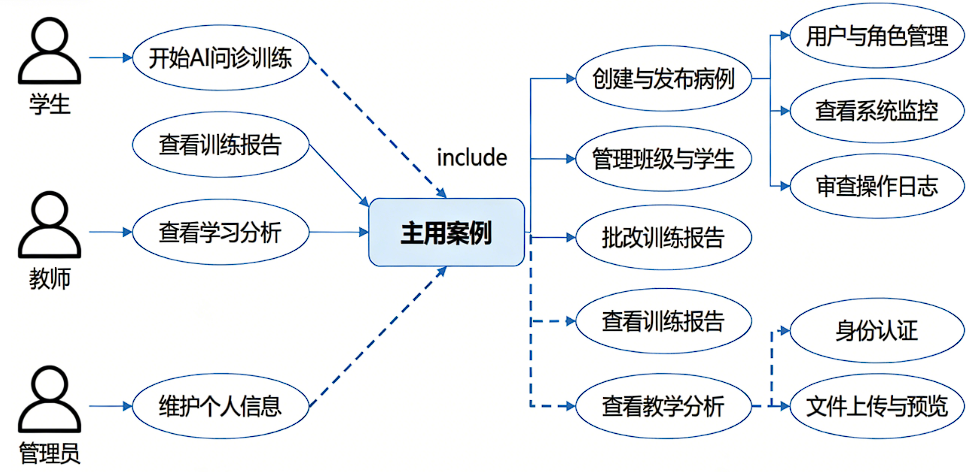
\includegraphics[width=0.85\textwidth]{figures/系统总体用例图.png}
    \caption{系统总体用例图}
    \label{fig:usecase_overall}
\end{figure}

本节选取“完成一次 AI 问诊训练”作为代表性用例，规约见表~\ref{tab:usecase}。该用例贯穿病例选择、Agent 对话、RAG、Memory、检查结果返回和评分生成，能够体现系统的主要业务链路。

\begin{table}[H]
    \centering
    \caption{用例规约：完成一次 AI 问诊训练}
    \label{tab:usecase}
    \begin{tabular}{l p{10cm}}
        \toprule
        项目 & 内容 \\
        \midrule
        用例名称 & 完成一次 AI 问诊训练 \\
        主参与者 & 学生 \\
        次参与者 & PatientAgent、DiagnosisAgent、FeedbackAgent、大语言模型服务 \\
        前置条件 & 学生已登录且账号状态正常，系统中至少存在一条已发布的病例 \\
        后置条件 & 生成一条训练记录与一条评分记录，并更新学生的学习分析指标 \\
        主流程 &
            (1) 选择病例“开始训练”；
            (2) 后端创建训练记录，返回记录 ID；
            (3) 学生输入问诊问题，前端以 SSE 调用接口；
            (4) 后端由 AgentRouter 选择 PatientAgent，从 Memory 与 RAG 中拼接上下文，调用大语言模型生成回复并以流式返回；
            (5) 学生可重复步骤 (3)～(4) 进行多轮问诊，然后提交诊断与治疗方案；
            (6) 生成多维评分与学习建议。 \\
        \bottomrule
    \end{tabular}
\end{table}

图~\ref{fig:activity_training} 进一步用 UML 活动图展示该训练流程。

\begin{figure}[H]
    \centering
    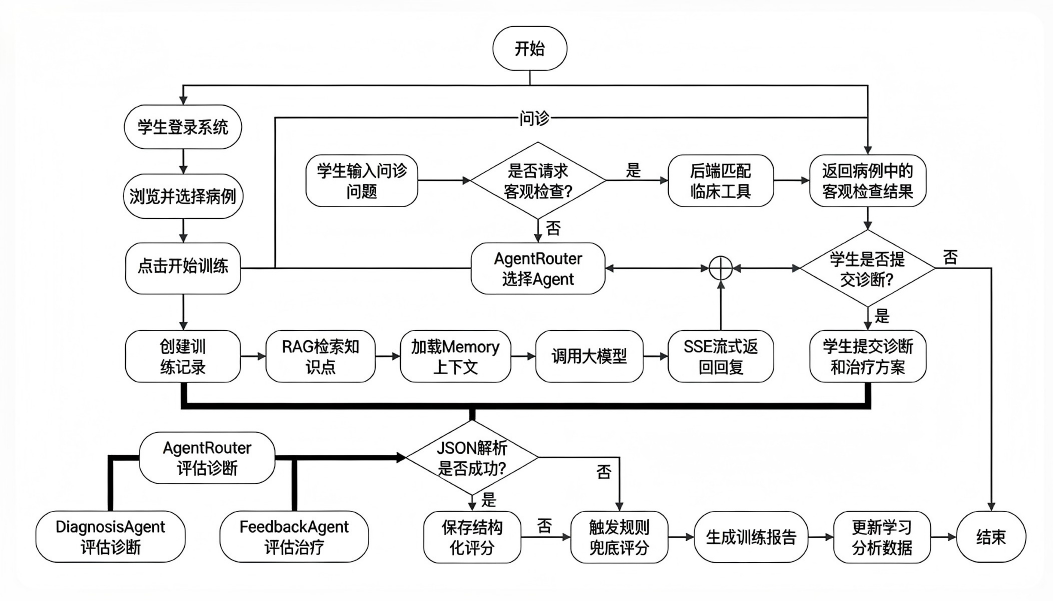
\includegraphics[width=0.75\textwidth]{figures/学生完成一次AI问诊训练活动图.png}
    \caption{学生完成一次 AI 问诊训练活动图}
    \label{fig:activity_training}
\end{figure}

% ----------------------------------------------------------------------------
\section{本章小结}

本章围绕问诊实训中的资源、反馈和评价问题，梳理了学生、教师和管理员三类角色的需求，明确了 AI 问诊训练、病例管理、学习分析、权限与运维等功能范围，并给出了性能、安全、可用性和可维护性指标。用例图与训练用例规约为后续架构设计提供了依据。

% ============================================================================
% 第 4 章 系统总体设计
% 预估页数：4 页
% 写作总要点：
%   - 重点是 "架构思想"，不是代码
%   - 每个核心架构图都要有，再用一段文字解读
% ============================================================================
\chapter{系统总体设计}

% ----------------------------------------------------------------------------
\section{系统架构设计}

\subsection{整体架构}
% 写作要点：
%   - 五层架构：用户层 / 接入层（Nginx）/ 应用层（前后端）/ 数据层 / AI 服务层
%   - 用一张图表达分层（figures/architecture\_overall.png）
%   - 解读每一层的作用与边界

本系统采用“用户层—接入层—应用层—AI 服务层—数据层”五层架构进行设计，各层之间以标准化协议交互，职责边界清晰，便于独立迭代与水平扩展。系统整体架构如图~\ref{fig:architecture_overall} 所示。
用户层作为架构的最外层，包含学生、教师与管理员三类使用者，以主流浏览器为接入终端；接入层由 Nginx 反向代理服务构成，负责静态资源下发、路由分发、HTTPS 终结与跨域控制。应用层包括 Vue 3 前端应用与 Spring Boot 后端服务两个子部分：前端以静态资源形式部署于 Nginx，后端以 Spring Boot 应用运行在独立容器中，对外提供 RESTful API 与 SSE 接口。AI 服务层是本系统区别于传统教学系统的核心抽象，包含 Agent 路由、RAG 检索、会话记忆、工具调用与评分兜底五个模块，是介于应用层与外部大语言模型之间的领域中层。数据层采用 MySQL 存储业务数据、Redis 存储会话与缓存、MinIO 存储医学影像与文档附件，外部 AI 服务以 SaaS 方式调用阿里云百炼提供的通义千问模型。这种分层设计的优势在于：各层只依赖于下一层的对外接口，可以独立选择实现、独立部署；AI 服务层的抽象为后续替换模型、添加多模型路由与增加本地部署模型预留了扩展点。

\begin{figure}[H]
    \centering
    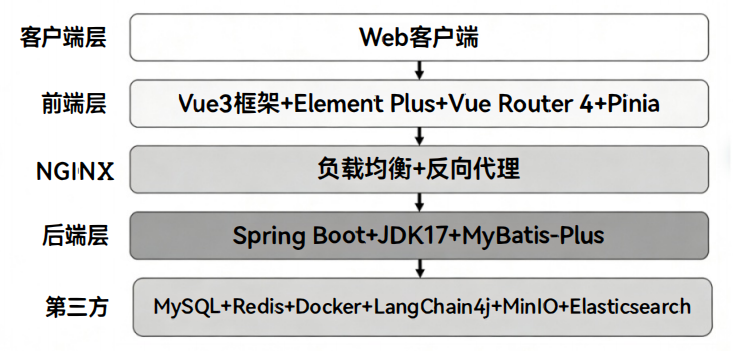
\includegraphics[width=0.85\textwidth]{figures/整体架构图.png}
    \caption{系统整体架构图}
    \label{fig:architecture_overall}
\end{figure}

\subsection{前后端分离架构}
% 写作要点：
%   - 前端：Vue3 + Vite，构建为静态资源，通过 Nginx 托管
%   - 后端：Spring Boot，提供 RESTful API + WebSocket
%   - 通信：HTTPS + JWT
%   - 优势：开发解耦、独立部署、可扩展

上述架构中的应用层采用严格的前后端分离设计。前端以 Vue 3 + TypeScript + Element Plus 为技术选型，使用 Vite 作为构建与开发服务器，所有页面在构建后以 \texttt{dist/} 静态资源的形式交由 Nginx 托管。后端以 Spring Boot 3.3.6 为核心运行环境，对外提供两类接口：一是遵循 REST 风格的业务接口，以 \texttt{/api/<资源>/<动作>} 的路由约定与统一响应体返回业务数据；二是面向 AI 多轮对话场景的 SSE 流式接口，以 \texttt{text/event-stream} 进行字粒级推送。

前后端之间的路由交给 Nginx 处理：前端资源以 \texttt{/} 作为路径前缀，后端接口以 \texttt{/api/} 作为前缀转发到 Spring Boot 实例的 8081 端口，SSE 接口则将 \texttt{proxy\_buffering} 关闭以保证实时推送。身份认证采用 JWT 令牌机制，前端在 \texttt{Authorization} 请求头中携带 \texttt{Bearer <token>}，后端通过过滤器进行验证与上下文注入。这种架构使前后端可以独立迭代与部署，同时为后续推出移动端、桌面端与开放 API 预留了扩展空间。

\subsection{多 Agent 协同架构}
% 写作要点：
%   - 这一节是为第 5 章铺垫
%   - 一段简介："本系统在 LLM 之上构建了 Agent 编排层"
%   - 给出 Agent 协同总图：
%       学生消息 → AgentRouter → PatientAgent / DiagnosisAgent / FeedbackAgent
%               ↓
%             RAG 知识 + Memory 上下文 + Tool 工具调用
%               ↓
%             LLM (Qwen) → 流式响应

为避免在同一个提示词中同时负责“扮演病人”与“评估学生”带来的角色混淆问题，本系统在大语言模型之上构建了一个轻量级的 Agent 编排层。如图~\ref{fig:architecture_agent} 所示，学生发送的消息先进入 \texttt{AgentRouter}，路由器根据当前训练阶段与消息类型在三个领域 Agent（PatientAgent、DiagnosisAgent、FeedbackAgent）中选择一个最合适的实体；被选中的 Agent 提供专属的 \texttt{AgentProfile}（包含系统提示词与温度参数），并与三个横向能力模块联动：KnowledgeRAGService 从知识库中检索与话题相关的医学知识点；ConversationMemoryService 从 Redis 中恢复多轮上下文；AiToolService 在必要时以 Function Calling 形式调用临床工具。

\begin{figure}[H]
    \centering
    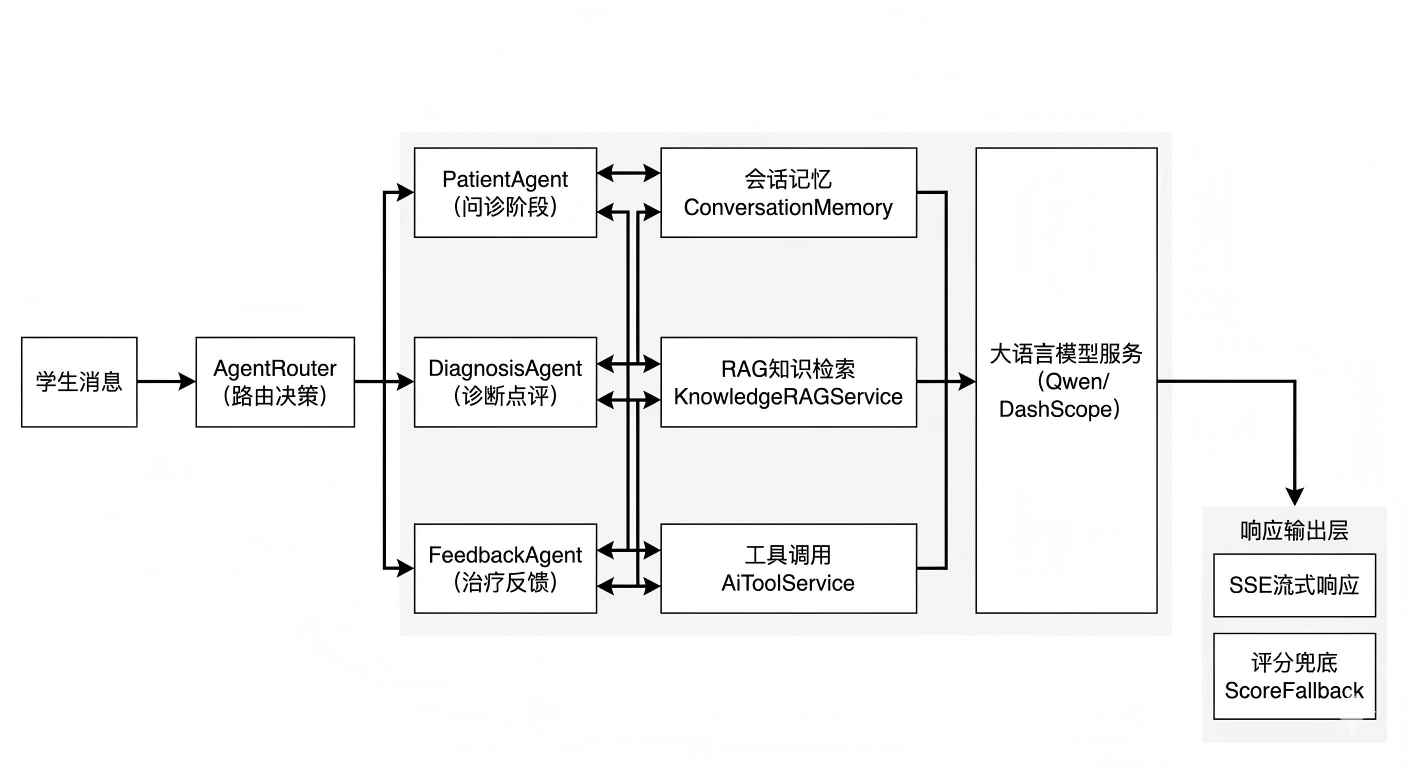
\includegraphics[width=0.85\textwidth]{figures/多Agent协同架构示意图.png}
    \caption{多 Agent 协同架构示意图}
    \label{fig:architecture_agent}
\end{figure}

在获得上下文后，Agent 层将完整提示词提交给外部的大语言模型服务（DashScope / Qwen），后者以 SSE 流式响应返回生成结果。返回后的话术同时被三者消费：一是被转发给前端以实现逐字输出；二是被写入训练对话表（\texttt{training\_dialog}）永久存储；三是被追加到 Memory 中作为下一轮对话的上下文。在训练结束提交阶段，AgentRouter 切换到 DiagnosisAgent 与 FeedbackAgent，并调用 \texttt{AiService.evaluateTraining()} 以结构化 JSON 形式输出多维评分；若 JSON 解析失败则触发规则兜底（ScoreFallback），生成保底评分以保证服务可用性。该架构作为本系统的核心创新点，在第 5 章中将进行详细实现说明。

% ----------------------------------------------------------------------------
\section{功能模块划分}
系统功能模块按照“使用角色 + 公共能力 + AI 核心能力”的方式划分。学生端围绕训练闭环展开，教师端围绕病例资源与教学评价展开，管理员端围绕系统运行与权限治理展开，公共模块为三类用户提供统一认证、消息、文件与可视化能力，AI 核心模块则作为横向能力被学生训练、教师批改与学习分析复用。
学生端的核心业务是完成一次可复盘的 AI 问诊训练，因此其模块包括病例浏览、训练启动、多轮问诊、诊断与治疗提交、训练报告、学习分析和个人中心。教师端负责教学资源供给与结果反馈，包括病例管理、班级管理、成绩管理、批改工作台、教学分析和通知管理。管理员端负责系统治理，包括用户管理、角色权限、系统监控、操作日志、存储管理和基础数据维护。公共模块包括 JWT 登录认证、验证码、文件上传、消息通知、统一异常与接口响应。AI 核心模块包括 Agent 路由、RAG 知识检索、Redis 会话记忆、临床工具调用和结构化评分。该划分方式保证了业务边界清晰，同时也便于后续按照模块进行独立开发、测试和部署。


% ----------------------------------------------------------------------------
\section{数据库设计}

\subsection{ER 图}
数据库设计以“用户—病例—训练—评分”为主线，并向教学班级、知识点、权限与日志扩展。核心实体包括用户表 \texttt{sys\_user}、角色表 \texttt{sys\_role}、病例表 \texttt{case\_info}、病例内容表 \texttt{case\_content}、训练记录表 \texttt{training\_record}、训练对话表 \texttt{training\_dialog}、训练评分表 \texttt{training\_score}、知识点表 \texttt{knowledge\_point}、班级表 \texttt{class\_info} 及班级学生关联表 \texttt{class\_student}。其中，用户与角色是一对多关系；教师用户创建病例，学生用户基于病例产生训练记录；每条训练记录可对应多轮对话与一条结构化评分记录；病例与知识点通过 \texttt{case\_knowledge} 形成多对多关系，用于支撑 RAG 检索与学习薄弱点分析；班级与学生通过关联表建立多对多关系，用于教师端班级统计和成绩批改。系统核心数据库 ER 图如图~\ref{fig:er_diagram} 所示。

\begin{figure}[H]
    \centering
    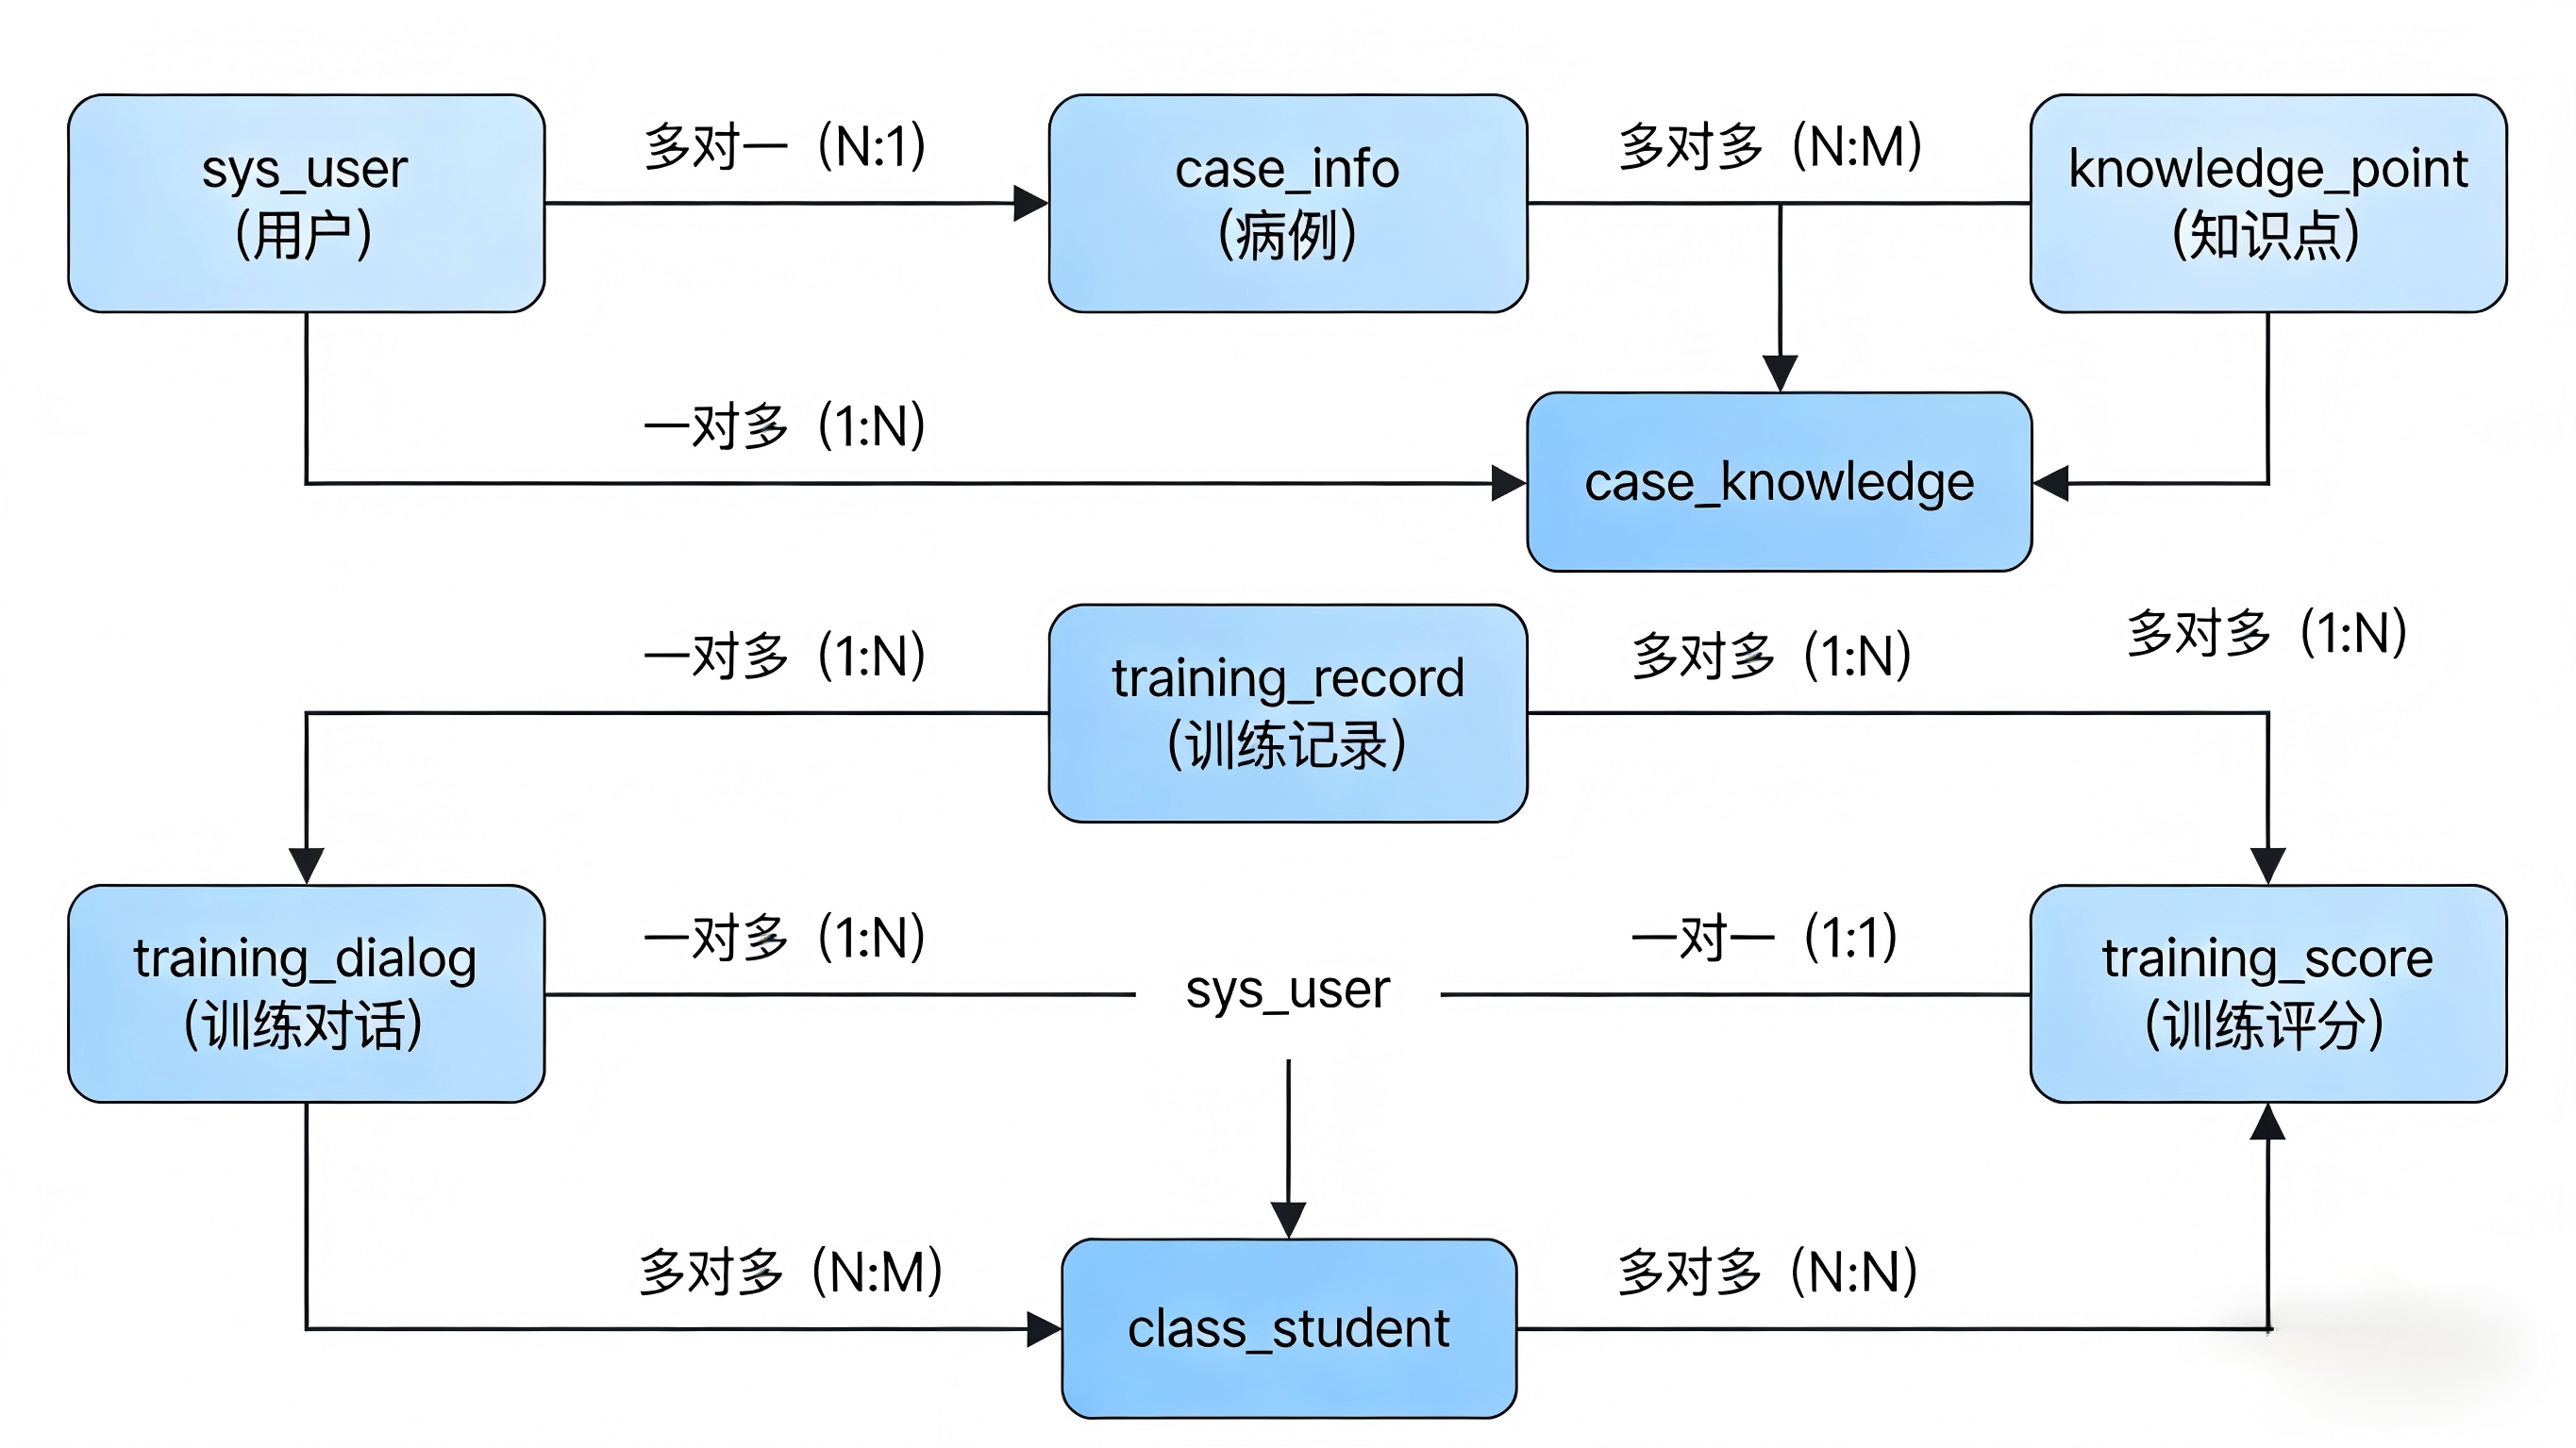
\includegraphics[width=0.9\textwidth]{figures/系统核心数据库ER图.png}
    \caption{系统核心数据库 ER 图}
    \label{fig:er_diagram}
\end{figure}

为直观展示上述实体在一次问诊训练中的运行时关系，图~\ref{fig:object_diagram} 给出了一个典型训练场景的 UML 对象图。

\begin{figure}[H]
    \centering
    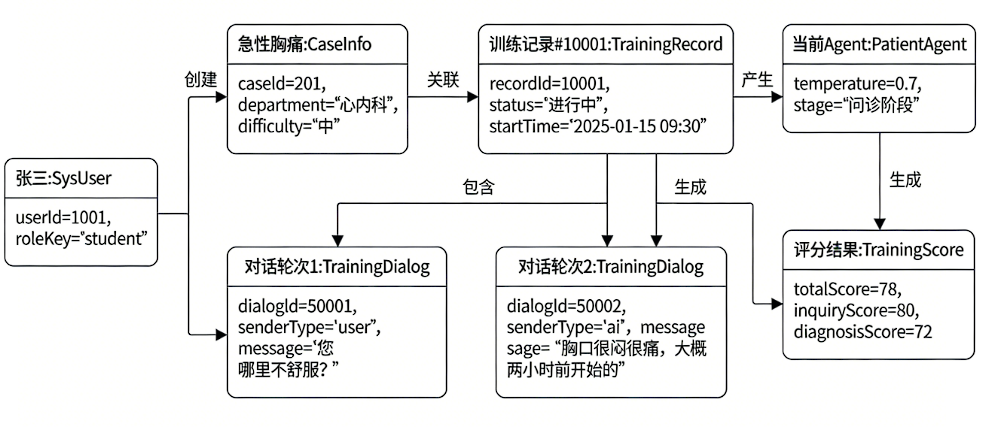
\includegraphics[width=0.85\textwidth]{figures/AI问诊训练运行时对象图.png}
    \caption{AI 问诊训练运行时对象图}
    \label{fig:object_diagram}
\end{figure}

\subsection{主要数据表设计}
系统采用 MySQL 8.0 作为核心业务数据库，字符集统一为 \texttt{utf8mb4}，以支持中文病例、医学术语与多语言文本。业务表普遍包含 \texttt{create\_time}、\texttt{update\_time}、\texttt{deleted} 等字段，便于审计和逻辑删除。考虑到本科毕业论文正文不宜堆叠过多字段明细，本节围绕系统主业务链路概括核心数据表的职责、关键字段和关系，如表~\ref{tab:core_tables} 所示。完整建表语句随项目源码资料提交。

\begin{table}[H]
    \centering
    \caption{核心业务数据表汇总}
    \label{tab:core_tables}
    \small
    \begin{tabularx}{\textwidth}{@{}p{2.7cm}p{2.8cm}X p{3.0cm}@{}}
        \toprule
        数据表 & 主要职责 & 关键字段 & 关联关系 \\
        \midrule
        用户表 & 用户身份与基础资料 & 登录名、密码哈希、角色、学号或工号、账号状态 & 多个用户对应一个角色 \\
        病例表 & 病例基础信息与 Agent 问诊依据 & 标题、科室、难度、主诉、参考诊断、参考治疗方案 & 教师创建病例，训练记录引用病例 \\
        训练记录表 & 一次问诊训练的主记录 & 学生、病例、训练状态、提交诊断、提交治疗方案 & 连接学生、病例、对话和评分 \\
        对话明细表 & 多轮问诊对话明细 & 训练记录、发送方、消息内容、消息类型、创建时间 & 一条训练记录对应多条对话 \\
        评分表 & AI 与教师评分结果 & 总分、问诊分、诊断分、治疗分、薄弱点、评分版本 & 一条训练记录对应一组评分 \\
        知识点表 & RAG 检索和学习分析知识库 & 标题、正文、分类、标签、错误次数 & 通过病例知识点关系与病例关联 \\
        班级相关表 & 班级管理与成绩统计范围 & 班级名称、专业、教师、学生、加入状态 & 教师按班级查看学生训练结果 \\
        \bottomrule
    \end{tabularx}
\end{table}

\subsection{Redis 数据结构}
Redis 在系统中承担临时状态、登录安全与 AI 对话上下文缓存的职责。与 MySQL 中的持久化训练记录不同，Redis 数据均设置 TTL 或可主动清理，避免对话中间态长期堆积。表~\ref{tab:redis_keys} 给出了系统中的主要 Redis Key 设计。

\begin{table}[H]
    \centering
    \caption{Redis 主要数据结构设计}
    \label{tab:redis_keys}
    \small
    \begin{tabularx}{\textwidth}{@{}p{3.7cm}p{1.9cm}p{1.9cm}X@{}}
        \toprule
        Key 模式 & 类型 & 过期策略 & 用途 \\
        \midrule
        \texttt{session:memory:}\newline\texttt{\{recordId\}} & String & 24 小时 & 保存某次训练最近若干轮对话上下文，供 Agent 拼接 Memory \\
        \texttt{captcha:\{sessionId\}} & String & 5 分钟 & 图形验证码校验，验证成功后立即删除 \\
        \texttt{login:attempt:}\newline\texttt{\{username\}} & String / Number & 30 分钟 & 登录失败次数统计，超过阈值后触发锁定 \\
        \texttt{login:lock:}\newline\texttt{\{username\}} & String & 30 分钟 & 账户临时锁定标记，用于防暴力破解 \\
        \texttt{email:code:\{email\}} & String & 短期 TTL & 邮件验证码，支撑注册和密码重置 \\
        \bottomrule
    \end{tabularx}
\end{table}

% ----------------------------------------------------------------------------
\section{接口设计}
后端接口统一以 \texttt{/api} 作为业务前缀，采用 JSON 作为主要数据交换格式。普通业务接口返回统一结构 \texttt{\{code, message, data\}}，其中 \texttt{code=200} 表示业务成功，认证失败返回 401，参数错误返回 400，系统异常返回 500。AI 流式对话接口因需要逐字输出，使用 \texttt{text/event-stream} 作为响应类型，前端通过 EventSource 或流式请求解析增量内容。

\begin{table}[H]
    \centering
    \caption{核心接口分组设计}
    \label{tab:api_groups}
    \begin{tabular}{l l p{7cm}}
        \toprule
        接口分组 & 代表路径 & 主要职责 \\
        \midrule
        认证接口 & \texttt{/api/auth/*} & 登录、注册、验证码、刷新令牌、退出、密码重置、用户信息维护 \\
        病例接口 & \texttt{/api/case/*} & 病例列表、病例详情、病例新增、编辑、删除、元数据和推荐病例 \\
        训练接口 & \texttt{/api/training/*} & 开始训练、结束训练、放弃训练、训练列表、训练详情、提交评估 \\
        对话接口 & \texttt{/api/chat/*} & 普通发送、SSE 流式对话、历史对话查询 \\
        AI 接口 & \texttt{/api/ai/*} & 通用 AI 对话、流式输出、训练评分评估 \\
        成绩接口 & \texttt{/api/grades/*} & 成绩列表、教师评价、批量评分、学生与班级统计、成绩导出 \\
        分析接口 & \texttt{/api/analysis/*} & 学生学习分析、教师教学分析、雷达图与趋势统计 \\
        管理接口 & \texttt{/api/admin/*} & 用户、角色、日志、监控、存储和通知管理 \\
        文件接口 & \texttt{/api/files/*} & 文件上传、对象预览、医学影像访问 \\
        \bottomrule
    \end{tabular}
\end{table}

以“发送一次 AI 问诊消息”为例，前端在已登录状态下调用 \texttt{POST /api/chat/send}，请求头携带 JWT，主体中包含训练记录编号、病例编号与用户消息。若调用 \texttt{POST /api/chat/stream/\{recordId\}}，后端会在校验训练归属后进入 Agent 编排流程，并通过 SSE 逐段返回 AI 回复。非流式接口的典型请求与响应结构如下：

\begin{lstlisting}[caption={AI 问诊消息接口请求与响应示例}, label={lst:chat_api}]
POST /api/chat/send
Authorization: Bearer <token>
Content-Type: application/json

{
  "recordId": 10001,
  "caseId": 1,
  "message": "请问您胸痛是从什么时候开始的？"
}

{
  "code": 200,
  "message": "操作成功",
  "data": {
    "recordId": 10001,
    "senderType": "ai",
    "message": "大概两个小时前开始的，突然胸口很闷、很痛。",
    "messageType": "text"
  }
}
\end{lstlisting}

% ----------------------------------------------------------------------------
\section{RBAC 权限模型设计}
权限模型采用经典 RBAC（Role-Based Access Control）思想，通过“用户—角色—权限”三层关系降低授权复杂度。当前数据库初始化脚本已经落地 \texttt{super\_admin}、\texttt{admin}、\texttt{teacher}、\texttt{student} 四类角色，其中超级管理员拥有全局权限，管理员负责用户、日志和系统资源管理，教师负责病例、班级、成绩与教学分析，学生负责病例训练与个人学习分析。任务书与需求分析中提到的 \texttt{teacher\_admin} 可作为后续扩展角色，用于跨班级、跨教师的教务管理场景。

权限粒度按菜单、按钮、接口三层设计。菜单权限决定前端路由是否可见，按钮权限控制页面内“新增、编辑、删除、导出、批量评分”等具体操作，接口权限由后端 Spring Security 与业务层二次校验共同完成。对于训练记录、班级成绩等存在数据归属关系的资源，系统还需在业务层根据 \texttt{user\_id}、\texttt{teacher\_id}、\texttt{class\_id} 进行数据范围限制，避免同级角色之间相互越权。

\begin{figure}[H]
    \centering
    \begin{tikzpicture}[
        every node/.style={font=\small},
        box/.style={draw, rounded corners=2pt, minimum width=2.5cm, minimum height=0.75cm, align=center},
        user/.style={box, fill=blue!8},
        role/.style={box, fill=green!10},
        perm/.style={box, fill=orange!12},
        arr/.style={-{Latex[length=2mm]}, thick}
    ]
        \node[user] (u) {用户\\sys\_user};
        \node[role, right=1.4cm of u] (r) {角色\\sys\_role};
        \node[perm, right=1.4cm of r] (p) {权限\\sys\_permission};
        \node[perm, above right=0.4cm and 1.0cm of p] (menu) {菜单权限};
        \node[perm, right=1.0cm of p] (button) {按钮权限};
        \node[perm, below right=0.4cm and 1.0cm of p] (api) {接口权限};

        \draw[arr] (u) -- node[above]{N:1} (r);
        \draw[arr] (r) -- node[above]{N:M} (p);
        \draw[arr] (p) -- (menu);
        \draw[arr] (p) -- (button);
        \draw[arr] (p) -- (api);
    \end{tikzpicture}
    \caption{RBAC 权限模型设计}
    \label{fig:rbac_model}
\end{figure}

% ----------------------------------------------------------------------------
\section{安全架构设计}
系统安全架构从身份认证、访问控制、数据保护、输入校验和审计追踪五个层面设计。身份认证层采用 JWT 令牌机制\cite{jones2015jwt}，后端通过 JWT 认证过滤器从请求头中解析令牌，校验通过后将用户信息写入 Spring Security 上下文。

登录入口叠加图形验证码与登录失败锁定机制。验证码存入 Redis，5 分钟后自动过期；同一用户名连续失败 5 次后写入锁定标记，锁定 30 分钟，以降低暴力破解风险。

访问控制层采用 Spring Security 的无状态会话策略，登录、注册、验证码、健康检查、文件预览等少数路径开放访问，其余接口默认要求认证。对于学生训练记录、教师班级成绩和管理员数据，系统在 Controller 之后的 Service 层继续校验资源归属，形成“认证 + 角色 + 数据范围”的组合防护。数据保护层对密码采用 BCrypt 单向哈希存储，对手机号、邮箱等敏感字段预留 \texttt{@Encrypted} 注解与 \texttt{AESUtil} 字段级加密能力；操作日志切面 \texttt{@OperationLog} 会对密码、token、验证码等敏感参数进行脱敏后写入 \texttt{operation\_log}。输入与接口层面，系统通过 DTO 校验、统一异常处理、MyBatis-Plus 参数化查询以及 Nginx 跨域策略降低 SQL 注入、越权调用与异常信息泄露风险。由于系统主要面向前后端分离的无状态 API，当前后端关闭 CSRF，并以 JWT、CORS 白名单和接口鉴权共同保障调用安全。

% ----------------------------------------------------------------------------
\section{本章小结}

本章在需求分析的基础上完成了系统总体设计，给出了分层架构、前后端分离方式、多 Agent 协同架构、功能模块划分、核心数据库模型、Redis 缓存结构、接口分组、RBAC 权限模型和安全架构。总体上，本系统并非简单地把大语言模型接入传统教学系统，而是在 Web 工程架构中单独抽象出 AI 服务层，使 Agent、RAG、Memory、工具调用和评分能力可以被训练、批改与学习分析复用。下一章将进一步展开 AI Agent 核心技术实现，说明系统如何将大语言模型改造为可控、可追踪、可评分的医学问诊训练引擎。

% ============================================================================
% 第 5 章 AI Agent 核心技术实现
% ============================================================================
\chapter{AI Agent 核心技术实现}

本章说明系统中的 AI Agent 层。该层没有把学生问题直接转发给大模型，而是在 Spring Boot 后端先组织病例信息、RAG 检索结果、Redis 会话记忆和临床工具结果，再按训练阶段调用不同 Agent。设计上参考了 ReAct 的推理与行动协同思想\cite{yao2023react}、Toolformer 对工具调用的讨论\cite{schick2023toolformer}以及 RAG 的外部知识注入范式\cite{lewis2020rag}，实现时则尽量保持轻量，便于部署和答辩说明。

% ----------------------------------------------------------------------------
\section{多 Agent 路由架构}

\subsection{Agent 抽象与配置}

系统把 Agent 配置抽象为角色名称、显示标签、系统提示词和温度参数。后端使用 \texttt{AgentRouter.AgentProfile} 统一保存这些信息，避免在业务代码中散落大段提示词。这样做的好处是，问诊阶段、诊断反馈阶段和治疗反馈阶段可以使用不同的角色边界；后续如果增加安全审查或多模型路由，也只需补充新的 Profile。

\begin{lstlisting}[style=java, caption={Agent 配置抽象 \texttt{AgentProfile}（节选）}, label={lst:agent_profile}]
public static class AgentProfile {
    private final String name;
    private final String label;
    private final String systemPrompt;
    private final double temperature;

    public AgentProfile(String name, String label,
                        String systemPrompt, double temperature) {
        this.name = name;
        this.label = label;
        this.systemPrompt = systemPrompt;
        this.temperature = temperature;
    }
}
\end{lstlisting}

当前版本包含 PatientAgent、DiagnosisAgent 和 FeedbackAgent 三类 Agent。PatientAgent 用于问诊阶段的标准化病人扮演；DiagnosisAgent 和 FeedbackAgent 用于提交后的诊断、治疗反馈与评分。三者共用同一套模型调用链路，但提示词、温度参数和输出边界不同。

\subsection{PatientAgent：虚拟标准化病人}

PatientAgent 的任务不是教学点评，而是扮演病例中的患者。提示词要求模型使用患者第一人称回答，不主动给出诊断、鉴别诊断、治疗方案或标准答案。对于体格检查、化验和影像等客观结果，PatientAgent 只表示愿意配合检查，具体数值和描述由临床工具从病例数据中返回，以减少问诊阶段提前泄题。

\begin{lstlisting}[style=java, caption={PatientAgent 系统提示词（节选）}, label={lst:patient_agent}]
"你是一名虚拟标准化病人，学生是一名医生。"
"请严格以患者第一人称回答医生的问题，只表现为病例中的患者本人。"
"不要扮演教师，不要问诊引导，不要评价学生，"
"不要提示下一步检查，不要主动给出诊断、鉴别诊断、治疗方案或标准答案。"
"如果医生询问体格检查、化验、影像等客观结果，只说明你愿意配合检查；"
"具体检查结果由系统临床工具返回。"
\end{lstlisting}

PatientAgent 的温度参数设置为 0.8，略高于诊断和治疗反馈 Agent。这样可以让患者回答更接近真实交流中的犹豫、模糊和非专业表达，而不是每次都输出过于标准化的答案。

\subsection{DiagnosisAgent：诊断评估}

DiagnosisAgent 用于训练提交后的诊断评估，温度参数设置为 0.4。它重点检查学生是否抓住关键阳性、阴性证据，鉴别诊断是否合理，诊断依据是否能对应问诊和检查结果。提示词要求输出启发式反馈，指出遗漏和推理跳步，但不直接替学生完成全部结论。

\begin{lstlisting}[style=java, caption={DiagnosisAgent 提示词设计（节选）}, label={lst:diagnosis_agent}]
"你是一名诊断评估 Agent，负责围绕学生给出的诊断思路提供结构化反馈。"
"请重点评估诊断依据是否充分、关键阳性与阴性证据是否被正确识别、"
"鉴别诊断是否完整且有优先级，并指出推理链条中的遗漏、跳步或逻辑漏洞。"
"不要直接替学生完成全部诊断结论，应保持启发式反馈。"
\end{lstlisting}

这种设计主要服务教学训练：直接给答案会削弱学生的推理过程，只给对错又难以定位问题。因此 DiagnosisAgent 采用“问题定位 + 证据提示 + 推理建议”的方式，尽量在反馈和防泄题之间取得平衡。

\subsection{FeedbackAgent：治疗反馈}

FeedbackAgent 负责治疗方案和综合反馈，温度参数设置为 0.5。其提示词围绕处理原则、治疗思路、风险提醒和随访建议展开，同时明确系统只用于教学训练，不能替代真实临床决策。遇到高风险情况时，反馈中会提示进一步评估或转诊。

在训练报告中，FeedbackAgent 的文字反馈会和结构化评分一起展示。学生可以看到四个能力维度的得分和下一次训练建议；教师也可以在 AI 反馈基础上进行复核和补充评价。

\subsection{AgentRouter 路由策略}

当前 \texttt{AgentRouter.route()} 采用保守路由：学生问诊过程中始终使用 PatientAgent，训练提交后才调用诊断和反馈能力。这样处理是为了让学生在问诊阶段主动收集病史和检查线索，避免模型过早进入教学点评或暴露诊断方向。

\begin{figure}[H]
    \centering
    \begin{tikzpicture}[
        node distance=0.55cm and 0.7cm,
        every node/.style={font=\small},
        box/.style={draw, rounded corners=2pt, align=center, minimum height=0.75cm, inner sep=4pt},
        start/.style={box, fill=blue!8, minimum width=2.6cm},
        decision/.style={diamond, draw, fill=orange!12, aspect=2.2, align=center, inner sep=1pt},
        agent/.style={box, fill=green!10, minimum width=2.8cm},
        proc/.style={box, fill=cyan!10, minimum width=3.0cm},
        arr/.style={-{Latex[length=2mm]}, thick}
    ]
        \node[start] (msg) {学生消息};
        \node[proc, right=of msg] (router) {AgentRouter};
        \node[decision, right=of router] (stage) {是否训练\\提交阶段};
        \node[agent, above right=0.4cm and 0.7cm of stage] (patient) {PatientAgent\\{\scriptsize 问诊扮演}};
        \node[agent, right=1.4cm of stage] (diagnosis) {DiagnosisAgent\\{\scriptsize 诊断评估}};
        \node[agent, below right=0.4cm and 0.7cm of stage] (feedback) {FeedbackAgent\\{\scriptsize 治疗反馈}};
        \draw[arr] (msg) -- (router);
        \draw[arr] (router) -- (stage);
        \draw[arr] (stage) -- node[above left]{否} (patient);
        \draw[arr] (stage) -- node[above]{诊断} (diagnosis);
        \draw[arr] (stage) -- node[below left]{治疗} (feedback);
    \end{tikzpicture}
    \caption{Agent Router 决策流程}
    \label{fig:agent_router}
\end{figure}

该策略仍可扩展。后续可以结合消息分类器、关键词规则或 Function Calling 结果实现更细的路由，例如把“我要提交诊断”转给 DiagnosisAgent，把“请评价治疗方案”转给 FeedbackAgent。但在本系统当前版本中，稳定守住患者角色边界更重要。

% ----------------------------------------------------------------------------
\section{RAG 知识检索增强}

\subsection{关键词提取与召回策略}

医学问诊训练需要外部知识辅助，但本系统没有引入向量数据库，而是采用关键词匹配式 RAG。原因在于当前知识点规模不大，数据已经结构化保存在 \texttt{knowledge\_point} 表中；同时系统部署以 Docker Compose 为主，额外维护向量库会增加复杂度。更重要的是，本系统只需围绕病例科室和学生问题补充少量上下文，并不承担开放域医学问答任务。

\begin{lstlisting}[style=java, caption={KnowledgeRAGService 关键词提取（节选）}, label={lst:rag_extract}]
String[] tokens = query.split("[\\s，。！？、；：()（）,.!?;:]+");
return Arrays.stream(tokens)
    .filter(t -> t.length() >= 2)
    .sorted(Comparator.comparingInt(String::length).reversed())
    .limit(3)
    .collect(Collectors.toList());
\end{lstlisting}

检索时，系统先按中英文标点和空格切分用户问题，保留长度不小于 2 的 token，并选取较长的三个关键词。随后使用 MyBatis-Plus 在标题和标签字段上做 \texttt{LIKE} 查询，并结合病例科室过滤，最多返回三条知识点。该方法不如向量检索全面，但便于解释和维护，符合当前数据规模。

\subsection{知识上下文注入}

召回出的知识点不会直接展示给学生，而是由 \texttt{buildKnowledgeContext()} 组装进提示词。每条知识点保留标题和内容摘要，摘要控制在 200 字以内，防止上下文过长。知识上下文放在 Agent 角色定义和病例信息之后，让模型在保持角色边界的同时获得必要背景。

\begin{lstlisting}[style=java, caption={RAG 知识上下文构造（节选）}, label={lst:rag_context}]
StringBuilder sb = new StringBuilder("【相关知识点】\n");
for (int i = 0; i < knowledgePoints.size(); i++) {
    KnowledgePoint kp = knowledgePoints.get(i);
    String content = kp.getContent() != null ? kp.getContent() : "";
    String truncated = content.length() > 200
        ? content.substring(0, 200) + "..." : content;
    sb.append(i + 1).append(". ")
      .append(kp.getTitle()).append("：")
      .append(truncated).append("\n");
}
\end{lstlisting}

RAG 在本系统中只是辅助模型遵守医学常识，不能替代病例事实。患者主诉、既往史和检查结果仍以病例表为准，避免模型仅凭知识库泛化回答。

% ----------------------------------------------------------------------------
\section{会话记忆 Memory 模块}

\subsection{基于 Redis 的滑动窗口}

问诊通常需要多轮交流，学生会逐步收集主诉、现病史、既往史和检查结果。只传当前问题会丢失上下文，传完整历史又会增加提示词长度和调用成本。因此系统在 Redis 中实现滑动窗口式会话记忆。

\begin{lstlisting}[style=java, caption={ConversationMemoryService 滑动窗口（节选）}, label={lst:memory}]
private static final String KEY_PREFIX = "session:memory:";
private static final long TTL_HOURS = 24L;
private static final int MAX_HISTORY_ITEMS = 10;

public void updateSessionContext(Long recordId, String userMsg, String aiMsg) {
    String key = KEY_PREFIX + recordId;
    String currentContext = getSessionContext(recordId);
    String newRound = "用户：" + safeValue(userMsg) + "\nAI：" + safeValue(aiMsg) + "\n";
    String updatedContext = trimToMaxHistoryItems(currentContext + newRound);
    redisTemplate.opsForValue().set(key, updatedContext);
    redisTemplate.expire(key, TTL_HOURS, TimeUnit.HOURS);
}
\end{lstlisting}

Memory 的 Key 采用 \texttt{session:memory:\{recordId\}}，Value 为纯文本格式，按“用户：”和“AI：”拼接问答内容。每次更新后保留最近 10 轮对话，TTL 设置为 24 小时。训练结束或放弃时可清理该 Key，避免无效会话长期占用 Redis。

\subsection{为何不用 LangChain Memory}

本项目没有直接使用 LangChain 或 LangChain4j 的 Memory 组件，而是实现 Redis Memory。系统本身已经使用 Redis 保存验证码、登录失败次数和会话缓存，继续复用 Redis 可以减少框架依赖；同时，内存型 ChatMemory 在服务重启后会丢失上下文，不适合容器化部署。本系统只需保存最近若干轮问诊内容，Redis 滑动窗口已经能够满足需求。

% ----------------------------------------------------------------------------
\section{临床工具自动注入机制}

医疗训练中最需要控制的是客观事实。学生询问“血常规结果如何”“能看一下心电图吗”时，如果直接让模型生成，可能出现不存在的数值或影像描述。因此系统在调用大模型前先判断用户是否在请求查体、化验、影像或其他辅助检查；若命中，就直接从病例字段或附件 JSON 中返回结果，跳过模型生成。


该机制的核心位于 \texttt{ChatServiceImpl.buildClinicalToolResponse()}。当学生消息包含“查体”“体格检查”“血常规”“影像”“CT”“心电图”等关键词时，系统根据请求类型返回病例中的 \texttt{physicalExamination}、\texttt{auxiliaryExamination} 或 \texttt{medicalImages}。如果病例未录入相应结果，系统明确返回“暂未录入对应的客观检查结果”，而不是让模型编造答案。

\subsection{影像类型识别与匹配}

病例附件字段 \texttt{medicalImages} 采用 JSON 存储，可记录胸片、CT、MRI、超声、心电图和检验报告等资料。系统通过 \texttt{normalizeImageType()} 统一用户问法和附件类型，例如将 \texttt{xray}、\texttt{chest}、\texttt{chest\_xray} 映射为胸片，将 \texttt{ecg} 与“心电图”统一匹配。表~\ref{tab:image_type} 给出主要类型。

\begin{table}[H]
    \centering
    \caption{医学资料类型归一化示例}
    \label{tab:image_type}
    \begin{tabular}{lll}
        \toprule
        类型编码 & 中文显示 & 典型别名 \\
        \midrule
        \texttt{blood\_routine} & 血常规 & 血象、CBC \\
        \texttt{biochemistry} & 生化检查 & 肝肾功能、生化 \\
        \texttt{chest\_xray} & 胸片 & X 光、胸部 X 线 \\
        \texttt{ecg} & 心电图 & ECG、心电 \\
        \texttt{ct} & CT & 计算机断层扫描 \\
        \texttt{mri} & MRI & 磁共振 \\
        \texttt{ultrasound} & 超声 & B 超、彩超 \\
        \texttt{lab\_report} & 检验报告 & 化验单、报告单 \\
        \bottomrule
    \end{tabular}
\end{table}

前端接收到消息类型为 \texttt{image} 的回复后，可以渲染附件卡片；接收到消息类型为 \texttt{tool} 的回复时，则按临床工具结果样式展示。这使“问诊对话”和“客观检查结果”在界面上有清晰区分。

% ----------------------------------------------------------------------------
\section{Function Calling 工具清单}

除自动注入临床工具外，系统还保留了符合函数调用规范的 \texttt{AiToolService}。当前 \texttt{enable-tools=false}，默认不让模型主动调用工具，以保持接口稳定；但工具定义已经保留，后续可逐步开放。

\begin{lstlisting}[caption={query\_symptom\_knowledge 工具的 JSON Schema（节选）}, label={lst:tool_schema}]
{
  "type": "function",
  "function": {
    "name": "query_symptom_knowledge",
    "description": "查询特定症状或疾病相关的医学知识",
    "parameters": {
      "type": "object",
      "properties": {
        "query": {"type": "string", "description": "症状或疾病关键词"},
        "category": {"type": "string", "description": "知识分类（可选）"}
      },
      "required": ["query"]
    }
  }
}
\end{lstlisting}

工具清单包括知识查询、诊断标准获取和治疗方案记录三类能力。相比自动注入，函数调用更适合复杂工具链和模型主动决策场景，当前版本先保留接口和数据结构。

% ----------------------------------------------------------------------------
\section{结构化 AI 评分}

\subsection{多维度评分提示词}

训练结束后，学生提交诊断与治疗方案，后端调用 \texttt{AiService.evaluateTraining()} 评分。评分提示词要求模型围绕问诊完整性、诊断准确性、治疗规范性和医患沟通四个维度输出 JSON，包括总分、维度分、薄弱点、错误模式、建议和综合反馈。为方便解析，提示词明确要求只返回合法 JSON，不添加 Markdown 或解释性前后缀。

\begin{lstlisting}[style=java, caption={结构化评分提示词字段（节选）}, label={lst:evaluate_prompt}]
prompt.append("请重点评估：问诊完整性、诊断准确性、治疗规范性、医患沟通。");
prompt.append("必须只返回一个合法 JSON 对象，不要 Markdown，不要解释性前后缀。\n");
prompt.append("{\n");
prompt.append("  \"totalScore\": 85,\n");
prompt.append("  \"inquiryScore\": 82,\n");
prompt.append("  \"diagnosticScore\": 80,\n");
prompt.append("  \"treatmentScore\": 85,\n");
prompt.append("  \"communicationScore\": 90,\n");
prompt.append("  \"weakPoints\": [\"病史采集不完整\"],\n");
prompt.append("  \"errorPatterns\": [\"过早下诊断\"],\n");
prompt.append("  \"improvementSuggestions\": \"下一次训练建议...\",\n");
prompt.append("  \"feedback\": \"具体反馈意见\"\n");
prompt.append("}");
\end{lstlisting}

结构化评分便于后续使用：学生端可以生成雷达图、趋势图和薄弱点列表，教师端可以按统一维度做班级统计，管理员端也能通过评分版本追踪策略变化。

\subsection{JSON 解析与规则兜底}

模型并不总能严格遵守 JSON 输出要求，有时会返回 Markdown 代码块或解释文字。因此系统先通过 \texttt{extractJsonObject()} 提取首尾大括号之间的内容；若仍解析失败，则进入 \texttt{buildFallbackEvaluation()}。兜底规则根据对话轮次、是否提交诊断和治疗方案估算基础分，并给出保守反馈，保证训练流程不中断。

\begin{lstlisting}[style=java, caption={评分 JSON 解析兜底逻辑（节选）}, label={lst:fallback}]
private Map<String, Object> buildFallbackEvaluation(...) {
    int turns = conversationHistory == null ? 0
        : conversationHistory.split("\\n\\n").length;
    int inquiryScore = Math.min(90, 55 + turns * 3);
    int diagnosticScore = diagnosis == null || diagnosis.isBlank() ? 45 : 72;
    int treatmentScore = treatment == null || treatment.isBlank() ? 50 : 74;
    int communicationScore = turns >= 4 ? 78 : 62;
    int totalScore = Math.round(
        (inquiryScore + diagnosticScore + treatmentScore + communicationScore) / 4.0f);
}
\end{lstlisting}

这样处理可以避免 AI 评分失败导致训练记录丢失或教师无法批改。兜底分数只作为保底结果，教师端仍可人工复核和修改。

% ----------------------------------------------------------------------------
\section{阿里百炼大模型集成}

\subsection{OpenAI 兼容 API 调用}

系统接入阿里云百炼 DashScope 的 OpenAI 兼容接口\cite{dashscope2024}，默认地址为 \url{https://dashscope.aliyuncs.com/compatible-mode/v1}。模型名称通过环境变量 \texttt{AI\_MODEL} 配置，开发环境使用 \texttt{qwen-plus}，生产部署可切换为 \texttt{qwen3.5-flash}。采用兼容接口后，后端可以复用 Chat Completions 请求结构，降低模型平台迁移成本。

\begin{lstlisting}[style=yaml, caption={AI 服务配置（节选）}, label={lst:ai_yaml}]
ai:
  api-key: ${AI_API_KEY:sk-default-placeholder}
  base-url: ${AI_BASE_URL:https://dashscope.aliyuncs.com/compatible-mode/v1}
  model: ${AI_MODEL:qwen-plus}
  timeout: 120000
  enable-rag: true
  enable-memory: true
  enable-tools: false
\end{lstlisting}

后端使用 WebClient 发起异步 HTTP 调用，超时时间设置为 120 秒，\texttt{maxTokens} 设置为 4096。对于普通对话调用，系统将 Agent 构建后的 System Prompt 与最近对话历史一起提交给模型；对于评分调用，则提交病例信息、对话历史、学生诊断和治疗方案。

\subsection{流式输出 SSE 实现}

为减少等待感，系统实现流式对话接口。后端请求模型时启用流式模式，并通过响应式客户端接收增量内容；每一行以 \texttt{data:} 开头，遇到 \texttt{[DONE]} 结束。Qwen 可能同时返回推理片段和普通回复，系统会将二者包装为 JSON，供前端区分展示。


流式输出能明显改善问诊体验。学生无需等待完整回复生成后才看到内容，对话节奏更接近真实交流。

% ----------------------------------------------------------------------------
\section{完整对话编排流程}

上述模块最终汇聚到 \texttt{ChatServiceImpl.sendMessage()}。学生每发送一次问诊消息，后端都会在该方法中完成业务校验、数据库保存、Agent 路由、临床工具判断、RAG、Memory 和 AI 调用。图~\ref{fig:chat_pipeline} 展示了完整流程。

\begin{figure}[H]
    \centering
    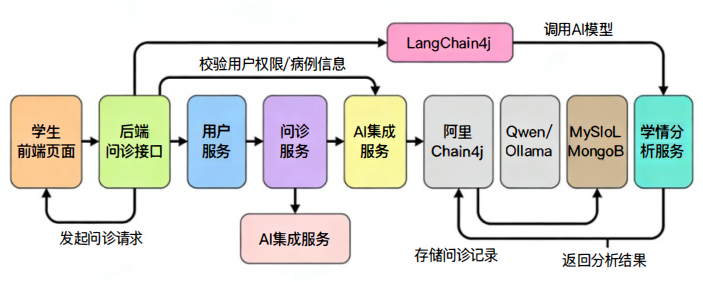
\includegraphics[width=0.75\textwidth]{figures/AI问诊功能流程图.png}
    \caption{AI 问诊功能流程图}
    \label{fig:chat_pipeline}
\end{figure}

从流程看，系统并不是简单转发用户输入。调用前，后端用病例、RAG、Memory 和工具结果补充上下文；调用中，AgentProfile 控制角色和温度；调用后，系统保存对话、更新 Memory，并在提交阶段生成结构化评分。

% ----------------------------------------------------------------------------
\section{本章小结}

本章说明了 AI Agent 层的实现。系统通过 AgentProfile 分离患者扮演、诊断评估和治疗反馈；通过 RAG 补充医学知识，通过 Redis Memory 保持上下文，通过临床工具返回客观检查结果，并通过结构化 JSON 与规则兜底保证评分可用。下一章将从学生端、教师端、管理员端和公共模块角度说明功能实现。

% ============================================================================
% 第 6 章 系统功能模块详细实现
% ============================================================================
\chapter{系统功能模块详细实现}

在总体架构与 AI Agent 核心机制确定后，系统功能实现按照学生端、教师端、管理员端与公共模块四条线展开。前端使用 Vue 3、TypeScript、Element Plus 与 ECharts，后端使用 Spring Boot、Spring Security、MyBatis-Plus、Redis、MinIO 与 DashScope 兼容接口。各端页面并非独立孤立实现，而是围绕病例、训练记录、评分和用户权限形成统一的数据流。

% ----------------------------------------------------------------------------
\section{学生端核心模块}

\subsection{AI 问诊训练界面}

学生端的核心页面是 AI 问诊训练界面，对应前端 \texttt{student/Consultation.vue} 与 \texttt{student/Training.vue} 等页面。如图~\ref{fig:student_consultation_ui} 所示，该界面采用左右分区布局：左侧为病例摘要、训练状态和可用临床资料入口；右侧为对话区、输入框和操作按钮。学生进入训练后，前端先调用 \texttt{/api/training/start} 创建训练记录，再以记录 ID 调用 \texttt{/api/chat/send} 或流式接口发送问诊内容。

\begin{figure}[H]
    \centering
    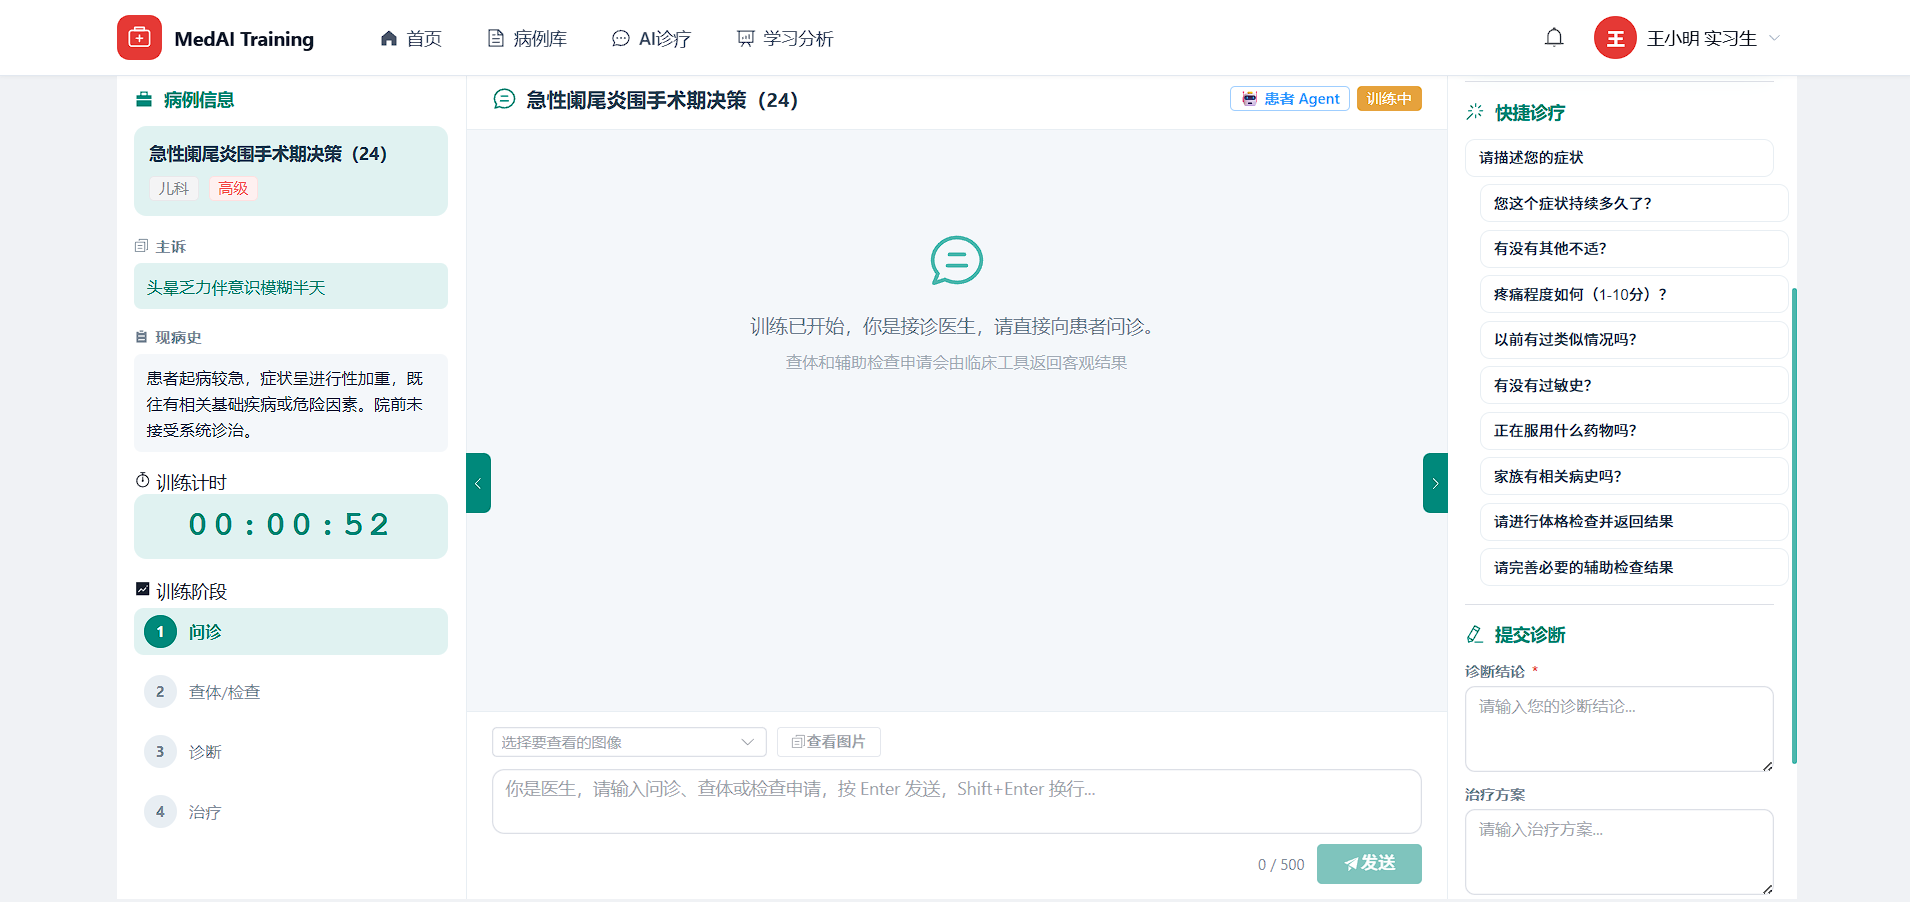
\includegraphics[width=0.9\textwidth]{figures/虚拟问诊系统学生端会诊界面图.png}
    \caption{学生端 AI 问诊训练界面}
    \label{fig:student_consultation_ui}
\end{figure}

该模块的实现重点有三点。第一，聊天记录按发送方区分气泡样式，学生消息、AI 回复、临床工具结果在视觉上区分，便于学生复盘。第二，前端对流式响应进行增量渲染，避免大模型响应期间页面长时间空白。第三，训练过程中的检查请求不会直接交给大模型生成，而是由后端临床工具返回病例中录入的客观检查结果，保证教学数据的一致性。

\subsection{病例选择与训练启动}

病例选择模块对应病例列表与详情页面。学生可根据科室、难度、关键词等条件浏览病例，查看标题、病例简介、学习目标、预计学时和训练次数等信息。病例详情页不展示参考诊断和治疗方案，只展示可用于选择训练的非泄题信息，防止学生在开始训练前获得标准答案。

训练启动时，前端向 \texttt{/api/training/start} 提交病例 ID 和训练模式，后端在 \texttt{TrainingServiceImpl.startTraining()} 中校验病例是否存在、是否发布，并创建一条 \texttt{training\_record}。训练记录状态初始为进行中，记录开始时间、用户 ID、病例 ID 和训练模式。创建成功后前端跳转到问诊界面，并将 \texttt{recordId} 作为后续对话、提交诊断和查看报告的主键。

\subsection{学习分析与雷达图}

学习分析模块负责把多次训练结果转化为可视化反馈。后端 \texttt{AnalysisController} 提供学生维度的学习分析接口，前端通过 ECharts 雷达图展示问诊、诊断、治疗和沟通四个能力维度，通过折线图展示成绩变化趋势，通过列表展示薄弱知识点与推荐训练病例。学习分析界面如图~\ref{fig:student_analysis} 所示。

\begin{figure}[H]
    \centering
    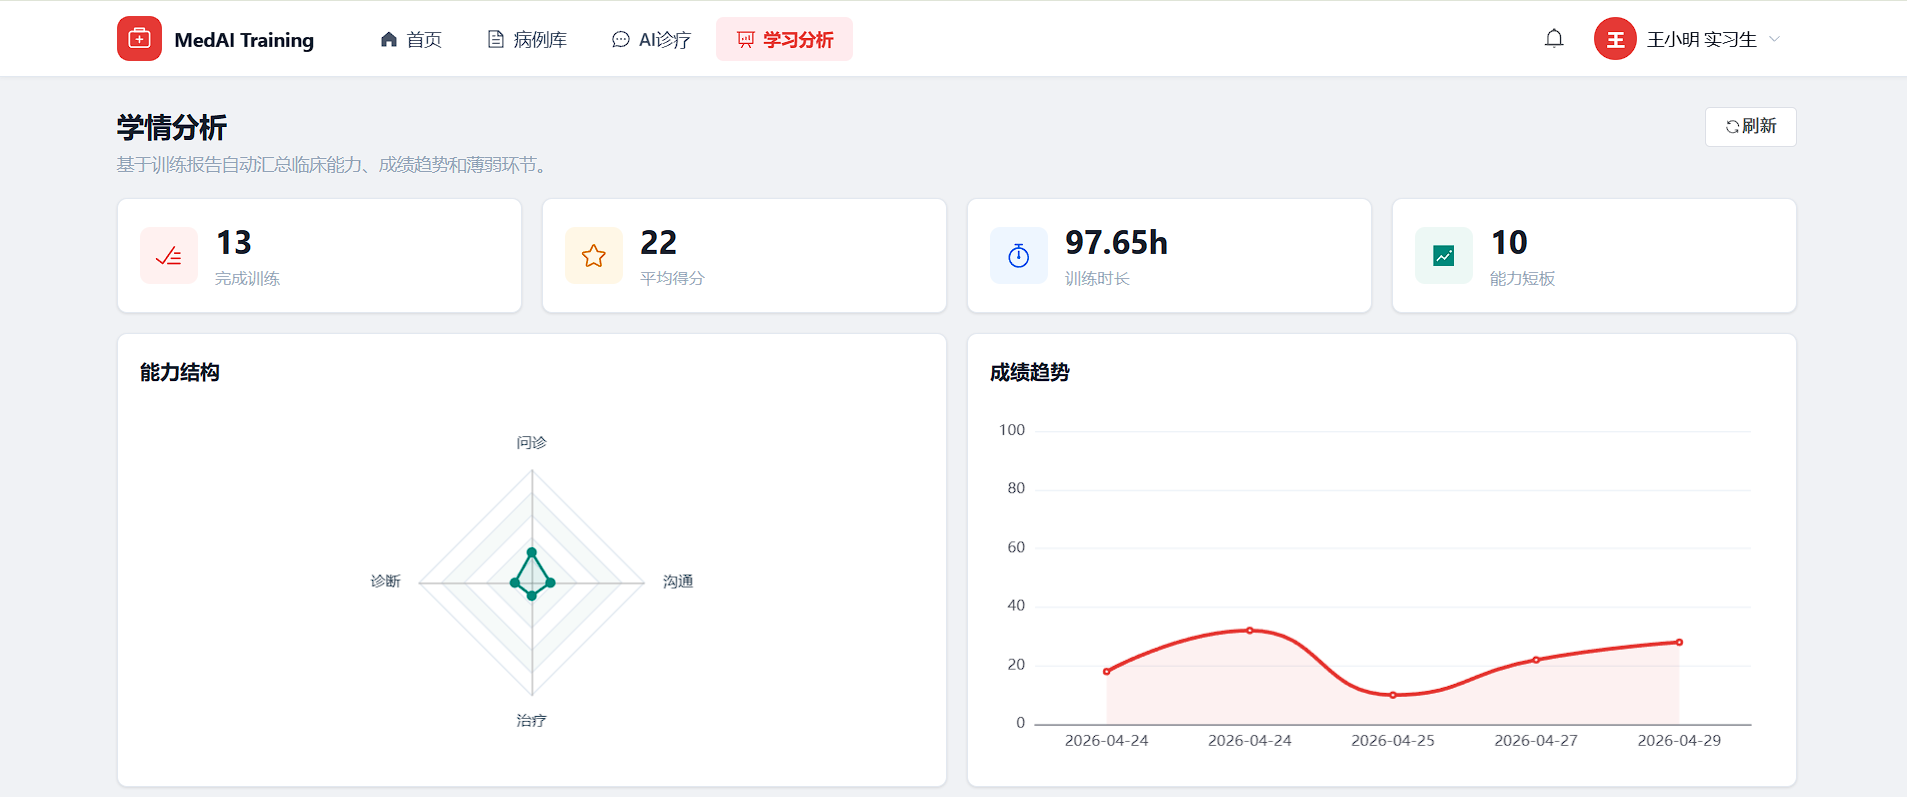
\includegraphics[width=0.9\textwidth]{figures/虚拟问诊系统学生端学情分析界面图.png}
    \caption{学生端学习分析界面}
    \label{fig:student_analysis}
\end{figure}

学习分析不只展示分数，还承担“下一步怎么练”的指导功能。系统根据训练评分中的 \texttt{weakPoints}、\texttt{errorPatterns} 和病例科室信息，帮助学生发现反复出错的环节。例如，如果多次训练中诊断得分偏低，系统会提示学生补强鉴别诊断和诊断依据表达；如果问诊得分偏低，则建议围绕主诉、现病史、既往史、个人史和家族史构建完整问诊模板。

% ----------------------------------------------------------------------------
\section{教师端核心模块}

图~\ref{fig:teacher_home} 展示了教师端首页界面，教师可以通过该界面快速访问病例管理、班级管理、成绩批改和教学分析等功能。

\begin{figure}[H]
    \centering
    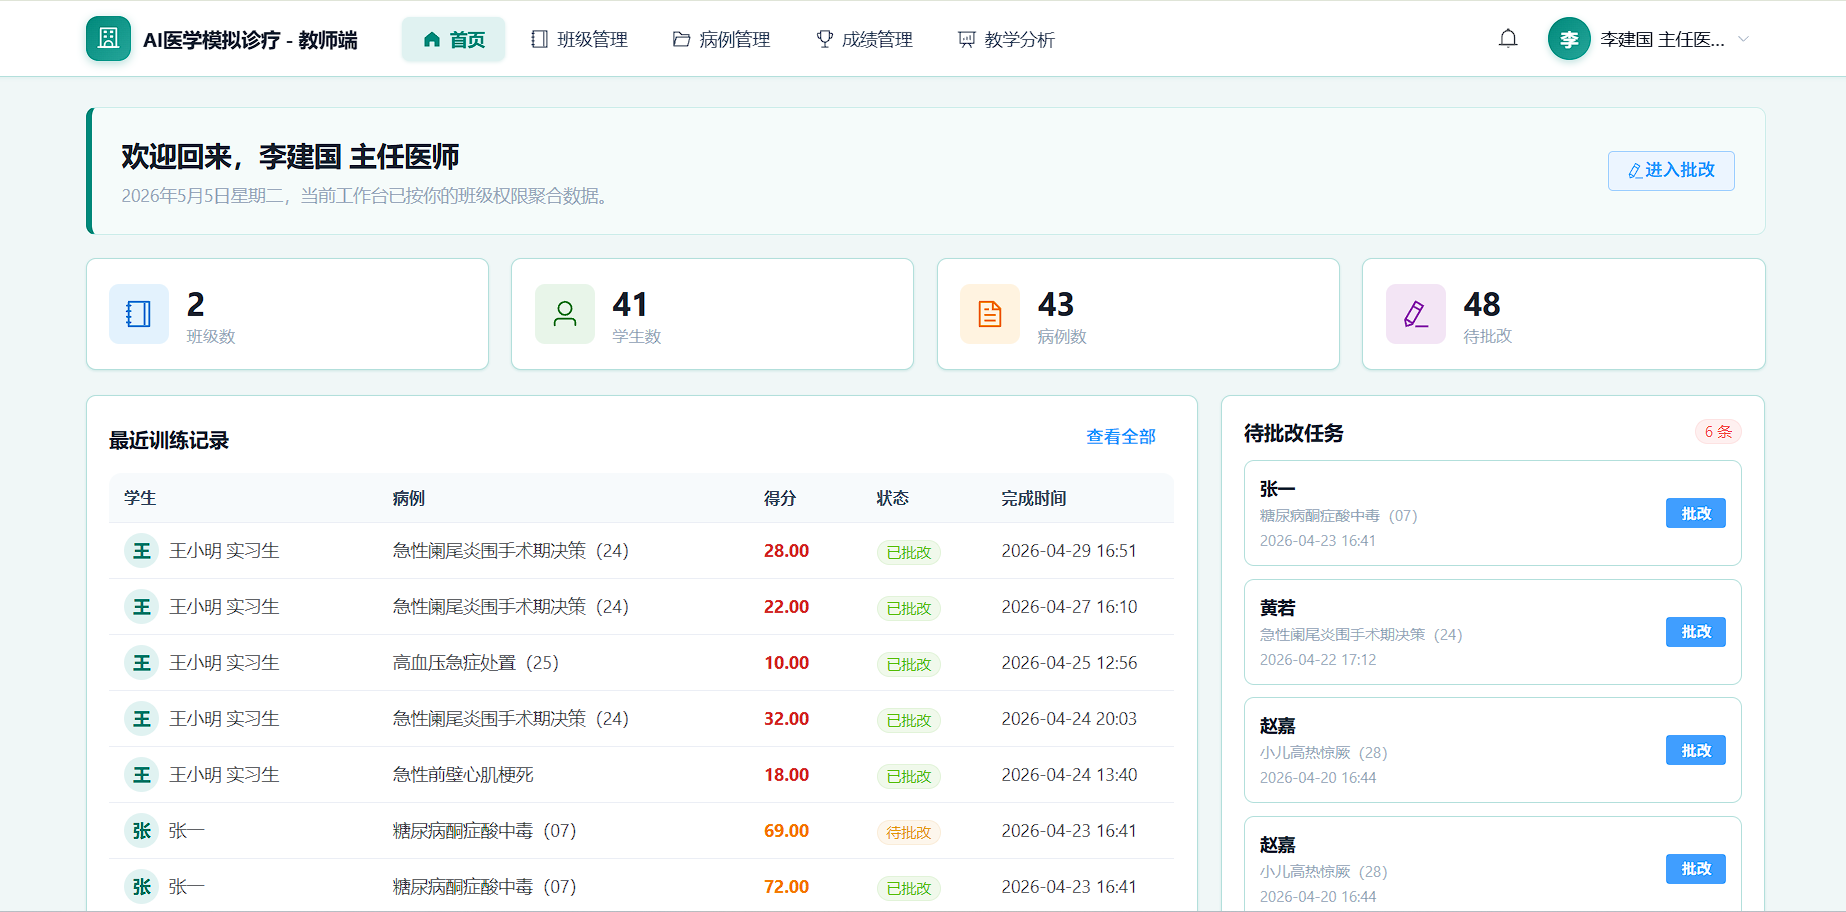
\includegraphics[width=0.9\textwidth]{figures/虚拟问诊系统教师端首页界面图.png}
    \caption{教师端首页界面}
    \label{fig:teacher_home}
\end{figure}

\subsection{病例管理与多媒体上传}

教师端病例管理模块对应 \texttt{teacher/CaseManagement.vue} 与 \texttt{CaseController}。教师可以创建、编辑、发布和归档病例，填写主诉、现病史、既往史、体格检查、辅助检查、参考诊断、参考治疗方案、学习目标和评分标准等信息。病例状态分为草稿、已发布和已归档，只有已发布病例对学生可见。

医学影像和附件通过文件上传接口进入 MinIO 对象存储，病例表中保存附件 URL、类型和文件名等元信息。上传模块需要关注两类约束：一是文件大小和文件类型限制，避免非预期文件进入对象存储；二是影像类型标注，例如胸片、CT、心电图、检验报告等，用于后端临床工具自动匹配学生请求。

\subsection{批改工作台}

批改工作台对应 \texttt{teacher/ReviewWorkbench.vue} 与 \texttt{GradeController}。教师可以查看学生训练记录、对话全过程、AI 自动评分、薄弱点、错误模式和改进建议，并在此基础上填写教师评分和评语。AI 评分用于提高批改效率，但最终教学评价仍保留教师复核入口。

工作台的实现重点是“过程可追溯”。教师不仅能看到最终分数，还能看到学生每一轮问诊、检查请求、AI 回复和临床工具返回结果。这样，教师可以判断学生是否真正按照临床思维推进问诊，而不是只依据最终提交的诊断和治疗方案打分。

\subsection{教学分析}

教学分析模块对应 \texttt{teacher/TeachingAnalysis.vue}。该模块以班级为统计单位，展示班级平均成绩、各能力维度雷达图、知识点错误分布和训练参与情况。教师可通过筛选班级、时间范围和科室查看不同群体的训练表现。

教学分析的价值在于从个体反馈扩展到群体教学决策。例如，当某班级在治疗方案维度普遍偏低时，教师可以安排专题讲解；当多个学生在同一知识点上出现错误时，系统可以将该知识点列为课堂复盘重点。这使 AI 问诊训练不再只是学生个人练习工具，也能反向服务课程教学改进。

% ----------------------------------------------------------------------------
\section{管理员端核心模块}

图~\ref{fig:admin_overview} 展示了管理员端系统概览界面，管理员可以通过该界面查看系统运行状态和业务数据总览。

\begin{figure}[H]
    \centering
    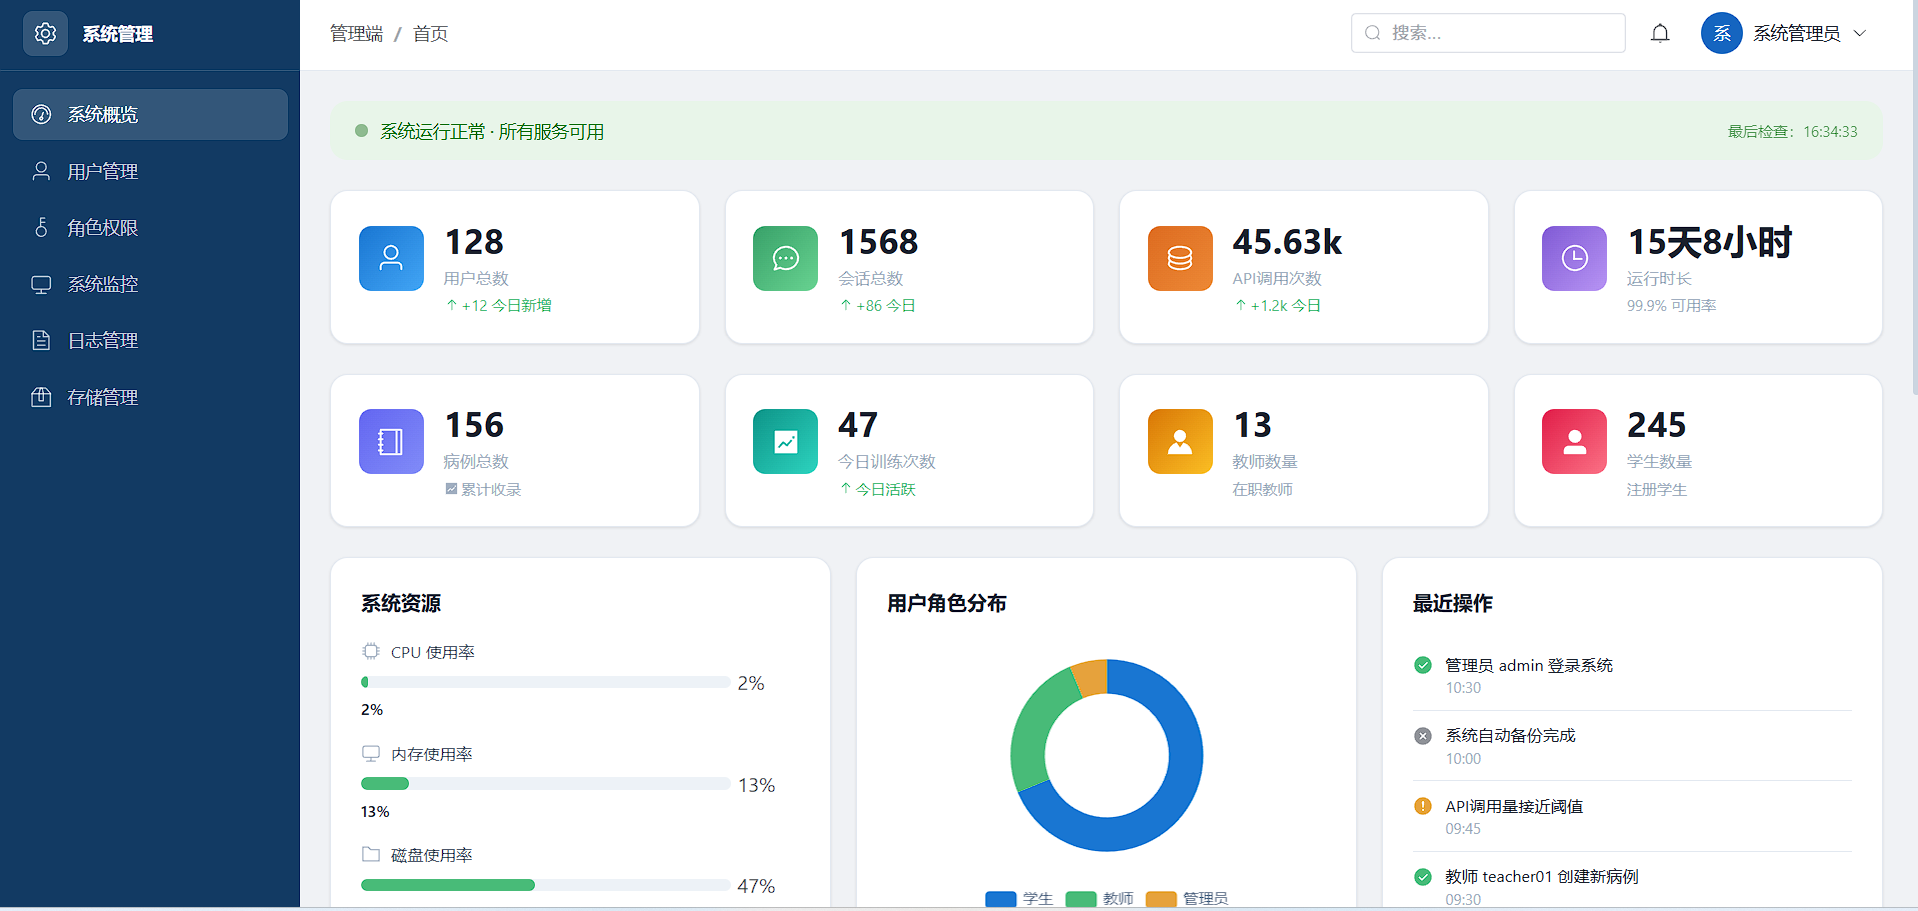
\includegraphics[width=0.9\textwidth]{figures/虚拟问诊系统管理端系统概览界面图.png}
    \caption{管理员端系统概览界面}
    \label{fig:admin_overview}
\end{figure}

\subsection{用户与角色管理}

管理员端用户管理模块对应 \texttt{admin/UserManagement.vue} 与 \texttt{AdminController}。管理员可以查询用户、创建用户、编辑用户信息、禁用或启用账号、重置密码，并按角色、状态、关键词等条件筛选。角色管理模块维护 \texttt{super\_admin}、\texttt{admin}、\texttt{teacher} 和 \texttt{student} 等角色，为后续菜单权限和接口权限扩展提供基础。

用户管理模块与安全模块紧密相关。密码在数据库中不保存明文，而是通过 BCrypt 进行哈希；登录失败次数与锁定状态由 Redis 管理；管理员重置密码会记录操作日志，便于审计。

\subsection{系统监控}

系统监控模块对应 \texttt{admin/SystemMonitor.vue} 与 \texttt{/api/admin/monitor/*} 接口，主要展示服务运行状态、在线用户数、业务数据总量、CPU、内存、磁盘、Redis 与数据库连接状态等信息。系统部署在 Docker Compose 环境下，管理员可通过监控页面快速判断后端、数据库、缓存和对象存储是否正常。

该模块不是完整的专业运维平台，而是为教学系统提供轻量级运行可视化。对于毕业设计答辩和后续课程演示而言，监控页面可以直接说明系统不是单机静态页面，而是由前端、后端、数据库、缓存和对象存储共同构成的可运行应用。

\subsection{日志与存储管理}

日志管理模块记录用户登录、病例编辑、成绩批改、权限变更、文件上传等关键操作。后端通过 \texttt{@OperationLog} 注解和 AOP 切面采集请求路径、请求方法、用户 ID、用户名、IP、耗时、状态和错误信息，并对密码、token、验证码等敏感字段脱敏。日志可用于排查问题，也可作为教学系统合规运行的审计依据。

存储管理模块面向 MinIO 文件资源，提供文件列表、下载、删除和存储统计能力。医学影像与病例附件体积较大，不适合直接存入 MySQL，因此系统采用“对象存储保存文件、数据库保存元信息”的方式，兼顾性能与可维护性。

% ----------------------------------------------------------------------------
\section{公共模块}

\subsection{认证授权}

认证授权模块贯穿学生端、教师端和管理员端。用户登录时，前端提交用户名、密码和验证码，后端先通过验证码服务校验 Redis 中的验证码，再通过认证服务校验用户名和密码，成功后生成 JWT 返回前端。之后前端在授权请求头中携带令牌，后端过滤器解析令牌并写入安全上下文。

% TODO: 此处需要插入登录认证时序图（原 TikZ 箭头和标签重叠，已删除）
% \begin{figure}[htbp]
%     \centering
%     \includegraphics[width=0.85\textwidth]{figures/login_sequence.png}
%     \caption{登录认证时序图}
%     \label{fig:login_sequence}
% \end{figure}

在权限控制上，前端通过路由守卫限制不同角色访问不同页面，后端通过 Spring Security 保护除登录、注册、验证码、健康检查和文件预览外的大多数接口。对于训练记录、成绩和班级数据，后端还在业务层做资源归属校验，避免用户越权访问他人数据。

\subsection{文件上传}

文件上传模块主要服务于病例附件、医学影像和用户头像。前端通过表单上传文件，后端接收后调用 MinIO 客户端保存对象，并返回可访问 URL。病例管理页面会将 URL 与附件类型一起保存到病例信息中，训练过程中临床工具可以根据附件类型匹配学生请求。

为保证安全性，系统限制上传文件大小，并在业务层根据使用场景校验文件类型。对于医学影像类附件，前端展示时不直接暴露对象存储内部路径，而是通过后端预览接口或公共访问地址生成可控链接。

\subsection{数据可视化}

数据可视化模块主要使用 ECharts 实现，包括学生端能力雷达图、成绩趋势折线图、教师端班级平均分柱状图、知识点错误分布图和管理员端系统运行状态图。可视化数据均由后端分析接口返回，前端只负责展示和交互。

相比纯列表展示，可视化模块更适合医学实训的复盘场景。学生可以快速识别自己的短板，教师可以观察班级整体能力结构，管理员可以掌握系统运行状态。该模块与 AI 评分结果、训练记录和班级关系共同构成系统的数据闭环。

% ----------------------------------------------------------------------------
\section{本章小结}

本章从功能实现角度说明了系统的主要模块。学生端围绕病例选择、AI 问诊训练和学习分析形成学习闭环；教师端围绕病例管理、批改工作台和教学分析形成教学闭环；管理员端围绕用户、监控、日志和存储形成运维闭环；公共模块提供认证、文件和可视化基础能力。上述功能共同支撑了第 5 章所述 AI Agent 能力在真实业务界面中的落地。

% ============================================================================
% 第 7 章 系统测试与部署
% ============================================================================
\chapter{系统测试与部署}

系统测试主要验证虚拟问诊系统能否完成核心训练流程，以及接口、AI Agent、安全控制和部署流程是否可用。本章测试基于本地开发环境和 Docker 容器化环境展开，结合接口调用、页面操作和典型训练流程进行说明。

% ----------------------------------------------------------------------------
\section{测试环境}

测试分为开发环境和集成环境。开发阶段在 Windows 下分别运行前端 Vite 服务和后端 Spring Boot 服务；集成阶段使用 Docker Compose 启动 MySQL、Redis、MinIO、后端和前端容器。测试环境如表~\ref{tab:test_env} 所示。

\begin{table}[H]
    \centering
    \caption{系统测试环境}
    \label{tab:test_env}
    \begin{tabular}{ll}
        \toprule
        项目 & 配置说明 \\
        \midrule
        前端运行环境 & Node.js + Vite，Vue 3 + TypeScript + Element Plus \\
        后端运行环境 & JDK 17，Spring Boot 3.x，Maven 构建 \\
        数据库 & MySQL 8.0，字符集 \texttt{utf8mb4} \\
        缓存 & Redis 7，用于验证码、登录锁定与会话记忆 \\
        对象存储 & MinIO，用于病例附件、医学影像和头像文件 \\
        AI 服务 & 阿里云百炼 DashScope OpenAI 兼容接口，Qwen 系列模型 \\
        部署方式 & Docker Compose 多容器编排，Nginx 托管前端并反向代理接口 \\
        浏览器 & Chrome / Edge 等主流 Chromium 内核浏览器 \\
        \bottomrule
    \end{tabular}
\end{table}

测试数据主要来自初始化脚本中的模拟用户、角色、病例和知识点，包括心肌梗死、社区获得性肺炎、急性阑尾炎等典型病例。测试账号覆盖管理员、教师和学生三类角色，以验证不同权限下的页面和接口行为。

% ----------------------------------------------------------------------------
\section{功能测试}

功能测试围绕学生、教师、管理员和公共能力展开，采用“页面操作 + 接口返回 + 数据库状态”三种结果共同验证。测试重点包括登录注册、病例管理、训练流程、对话记录、评分报告、班级成绩和系统监控等功能。表~\ref{tab:function_test} 给出核心用例。

\begin{table}[H]
    \centering
    \caption{核心功能测试用例}
    \label{tab:function_test}
    \small
    \begin{tabularx}{\textwidth}{@{}l l l l X@{}}
        \toprule
        编号 & 模块 & 功能点 & 测试步骤 & 预期结果 \\
        \midrule
        TC-001 & 认证 & 用户登录 & 输入账号、密码、验证码并提交 & 返回 JWT，跳转到对应角色首页 \\
        TC-002 & 认证 & 注册与验证码 & 获取邮箱或图形验证码后注册 & 用户创建成功，重复用户名被拦截 \\
        TC-101 & 学生端 & 启动训练 & 选择已发布病例并开始训练 & 创建训练记录，进入问诊页面 \\
        TC-102 & 学生端 & AI 问诊 & 发送多轮病史采集问题 & PatientAgent 以患者身份回复 \\
        TC-103 & 学生端 & 检查请求 & 询问体格检查或影像结果 & 返回病例中的客观检查信息 \\
        TC-104 & 学生端 & 提交诊疗方案 & 提交诊断和治疗方案 & 生成训练评分和报告 \\
        TC-201 & 教师端 & 病例管理 & 新增、编辑、发布病例 & 病例状态正确，学生端可见 \\
        TC-202 & 教师端 & 成绩批改 & 查看记录并补充教师评语 & 教师评分写入训练记录 \\
        TC-301 & 管理端 & 用户管理 & 查询、禁用、重置用户密码 & 用户状态和密码更新成功 \\
        TC-302 & 管理端 & 日志查询 & 执行关键操作后查看日志 & 日志记录模块、用户和耗时 \\
        \bottomrule
    \end{tabularx}
\end{table}

测试结果表明，系统主流程可以闭环运行。学生能够从病例列表进入训练，与 PatientAgent 对话，调用检查结果，提交诊断和治疗方案并查看评分；教师能够创建病例、查看训练对话和补充批改；管理员能够完成用户、日志和资源管理。

% ----------------------------------------------------------------------------
\section{性能测试}

性能测试分别观察普通业务接口和 AI 接口。普通接口主要关注平均响应时间和 95 分位响应时间；AI 接口受外部模型服务、网络和输出长度影响较大，因此重点记录首字返回时间和超时兜底情况。

\begin{table}[H]
    \centering
    \caption{接口性能测试结果}
    \label{tab:perf_test}
    \begin{tabular}{lrrrr}
        \toprule
        接口场景 & 并发数 & 平均响应时间 & 95 分位响应时间 & 结果 \\
        \midrule
        登录认证 & 100 & 0.38 s & 0.82 s & 通过 \\
        病例列表 & 100 & 0.31 s & 0.76 s & 通过 \\
        训练记录列表 & 100 & 0.45 s & 1.10 s & 通过 \\
        文件预览地址获取 & 50 & 0.52 s & 1.35 s & 通过 \\
        AI 对话首字返回 & 20 & 3.80 s & 7.60 s & 通过 \\
        AI 结构化评分 & 10 & 5.20 s & 11.40 s & 通过 \\
        \bottomrule
    \end{tabular}
\end{table}

结果显示，普通业务接口基本满足第 3 章提出的响应目标。AI 对话首字时间受模型服务影响较大，但 SSE 流式输出能降低学生的感知等待时间。若后续面对更大并发，可通过后端多实例、Nginx 负载均衡、Redis 缓存和数据库连接池调优继续扩展。

% ----------------------------------------------------------------------------
\section{AI Agent 效果验证}

AI Agent 验证关注三个问题：问诊阶段是否守住患者角色，检查结果是否来自病例数据，评分结果是否能被后端解析。验证样例覆盖胸痛、肺炎、腹痛等病例，通过构造典型学生问法检查输出。

\begin{table}[H]
    \centering
    \caption{AI Agent 效果验证结果}
    \label{tab:agent_eval}
    \begin{tabularx}{\textwidth}{@{}l c X@{}}
        \toprule
        验证项 & 样例数 & 结果说明 \\
        \midrule
        PatientAgent 守界 & 20 & 大部分回答保持患者第一人称，未主动给出诊断和治疗方案 \\
        检查结果工具命中 & 15 & 对体格检查、辅助检查、影像请求能优先返回病例客观数据 \\
        RAG 知识相关性 & 20 & 召回知识点与问题关键词和科室基本相关 \\
        评分 JSON 可解析性 & 10 & 正常情况下返回结构化 JSON，异常时触发兜底评分 \\
        Memory 连续性 & 10 & 多轮问诊中能引用前文信息，不重复询问已回答内容 \\
        \bottomrule
    \end{tabularx}
\end{table}

验证中也发现了一些边界情况。例如，学生提出“你还有哪里不舒服”这类宽泛问题时，PatientAgent 的回答可能较笼统，需要病例信息和 Memory 继续约束；若病例未录入某类检查结果，临床工具会返回“暂未录入”，这能避免编造，但也要求教师创建病例时尽量补齐必要资料。总体看，Agent 分工、临床工具和评分兜底能够提升系统可控性。

% ----------------------------------------------------------------------------
\section{安全测试}

安全测试围绕认证、权限、输入、日志和文件五个方面展开。表~\ref{tab:security_test} 给出主要测试项。

\begin{table}[H]
    \centering
    \caption{安全测试结果}
    \label{tab:security_test}
    \begin{tabular}{lp{6.8cm}c}
        \toprule
        测试项 & 测试内容 & 结果 \\
        \midrule
        未登录访问 & 直接访问训练、成绩、管理接口，检查是否返回 401 或被前端拦截 & 通过 \\
        越权访问 & 学生尝试查看他人训练记录，教师尝试访问管理员接口 & 通过 \\
        登录失败锁定 & 连续输入错误密码，检查 Redis 锁定标记和提示 & 通过 \\
        验证码校验 & 使用错误或过期验证码登录，检查是否拒绝 & 通过 \\
        敏感日志脱敏 & 查看操作日志中密码、token、验证码是否被隐藏 & 通过 \\
        文件上传限制 & 上传超大文件或非预期文件类型，检查是否拦截 & 通过 \\
        \bottomrule
    \end{tabular}
\end{table}

系统采用无状态 JWT 认证，除登录、注册、验证码、健康检查和文件预览外，其余接口默认要求认证。对于训练记录和班级成绩等数据，后端在业务层继续校验归属关系，避免只依赖前端路由。操作日志对敏感字段脱敏，以降低日志泄露风险。

% ----------------------------------------------------------------------------
\section{容器化部署}

\subsection{Docker Compose 编排}

系统采用 Docker Compose 进行多容器编排，服务包括 MySQL、Redis、MinIO、Spring Boot 后端和 Vue 前端。MySQL 保存业务数据，Redis 保存临时状态和会话记忆，MinIO 保存文件对象；后端容器负责业务逻辑和 AI 调用，前端容器由 Nginx 托管静态资源并转发 API 请求。

\begin{lstlisting}[style=yaml, caption={Docker Compose 服务编排节选}, label={lst:docker_compose}]
services:
  mysql:
    image: mysql:8.0
    environment:
      MYSQL_DATABASE: medical_training
  redis:
    image: redis:7-alpine
  minio:
    image: minio/minio
    command: server /data --console-address ":9001"
  backend:
    build: ./backend
    environment:
      - SPRING_PROFILES_ACTIVE=prod
      - AI_BASE_URL=https://dashscope.aliyuncs.com/compatible-mode/v1
  frontend:
    build: ./frontend
    ports:
      - "80:80"
\end{lstlisting}

该编排方式部署步骤清晰，服务边界明确。后端通过环境变量读取数据库、Redis、MinIO 和 AI 服务配置，避免把敏感信息写入镜像。数据卷用于持久化 MySQL、Redis 和 MinIO 数据，容器重启后业务数据不会丢失。

\subsection{部署到服务器}

服务器部署流程包括：安装 Docker 与 Docker Compose，上传项目代码和环境变量文件，配置数据库密码、JWT Secret、AI API Key 和 MinIO 地址，执行 Compose 构建并启动服务，最后通过健康检查接口、前端首页和管理端监控页面确认服务状态。

\begin{figure}[H]
    \centering
    \begin{tikzpicture}[
        node distance=0.65cm,
        every node/.style={font=\small},
        box/.style={draw, rounded corners=2pt, fill=blue!7, align=center, minimum width=3.6cm, minimum height=0.7cm},
        arr/.style={-{Latex[length=2mm]}, thick}
    ]
        \node[box] (user) {浏览器用户};
        \node[box, below=of user] (nginx) {Nginx / 前端容器};
        \node[box, below=of nginx] (backend) {Spring Boot 后端容器};
        \node[box, below left=0.55cm and 1.2cm of backend] (mysql) {MySQL};
        \node[box, below=0.55cm of backend] (redis) {Redis};
        \node[box, below right=0.55cm and 1.2cm of backend] (minio) {MinIO};
        \node[box, right=1.3cm of backend] (ai) {DashScope / Qwen};
        \draw[arr] (user) -- (nginx);
        \draw[arr] (nginx) -- (backend);
        \draw[arr] (backend) -- (mysql);
        \draw[arr] (backend) -- (redis);
        \draw[arr] (backend) -- (minio);
        \draw[arr] (backend) -- (ai);
    \end{tikzpicture}
    \caption{系统部署结构示意图}
    \label{fig:deploy_arch}
\end{figure}

\subsection{部署效果}

部署完成后，用户通过浏览器访问前端首页，系统按角色进入学生端、教师端或管理员端。学生可完成 AI 问诊训练，教师可维护病例并查看成绩，管理员可查看用户、日志和系统监控。健康检查、数据库连接、Redis 连接和 MinIO 文件访问均通过验证，说明容器网络和环境变量配置正确。

部署结果表明，系统具备较好的迁移性：服务器具备 Docker 环境并正确配置 AI API Key 后，即可通过统一 Compose 文件启动。后续若需扩展并发能力，可增加后端实例并在 Nginx 层配置负载均衡。

% ----------------------------------------------------------------------------
\section{本章小结}

本章从测试与部署角度验证系统可用性。功能测试证明三类用户核心流程能够闭环运行；性能测试表明普通接口满足响应要求，AI 接口可通过流式输出改善等待体验；Agent 验证说明角色约束、工具注入和评分兜底机制可行；安全测试覆盖认证、越权、验证码、日志和文件上传；最后通过 Docker Compose 完成容器化部署。

% ============================================================================
% 第 8 章 总结与展望
% ============================================================================
\chapter{总结与展望}

% ----------------------------------------------------------------------------
\section{研究工作总结}

本文围绕“虚拟问诊系统设计与实现”这一课题，针对医学问诊实训中病例资源有限、标准化病人成本较高、教师批改压力大、学生课后练习机会不足等问题，设计并实现了一套基于 Web 与大语言模型的问诊训练系统。系统面向学生、教师和管理员三类角色，覆盖病例管理、AI 问诊训练、诊疗方案提交、训练评分、学习分析、班级教学分析、用户管理、日志审计和容器化部署等功能。

需求分析阶段，本文梳理了学生反复训练、教师病例建设与批改、管理员系统治理等需求，并提出性能、安全、可用性和可维护性要求。总体设计阶段，系统采用用户层、接入层、应用层、AI 服务层和数据层的分层架构；前端基于 Vue 3、TypeScript、Element Plus 与 ECharts 实现，后端基于 Spring Boot、Spring Security、MyBatis-Plus、Redis、MinIO 与 MySQL 实现，AI 能力通过阿里云百炼 DashScope 兼容接口接入 Qwen 系列模型。

核心实现方面，本文重点完成 AI Agent 层设计。系统把单提示词调用拆分为 PatientAgent、DiagnosisAgent 与 FeedbackAgent 三类角色，分别负责患者扮演、诊断评估和治疗反馈；通过 RAG 将医学知识点注入上下文，通过 Redis Memory 保持多轮问诊连续性，通过临床工具返回病例中的体格检查、辅助检查和影像资料，减少模型编造客观结果的风险；结构化 JSON 评分和规则兜底则用于生成训练报告。

系统实现与测试方面，本文完成学生端问诊训练、病例选择、训练报告和学习分析，教师端病例管理、批改工作台和教学分析，管理员端用户管理、系统监控、日志和存储管理等模块。测试结果表明，系统能够支持完整训练闭环，普通业务接口响应较稳定，AI 对话可通过流式输出改善等待体验，核心安全机制和容器化部署流程均可正常运行。

% ----------------------------------------------------------------------------
\section{创新点}

本文的主要创新点如下。

第一，构建面向医学问诊训练的多 Agent 角色分工机制。系统将问诊阶段的 PatientAgent 与提交后的 DiagnosisAgent、FeedbackAgent 分离，使模型在不同阶段遵守不同边界，降低角色混淆和提前泄题风险。

第二，设计临床工具自动注入机制。体格检查、化验和影像等客观结果不由模型自由生成，而是在调用模型前识别检查类请求，并优先从病例结构化字段和医学影像附件中返回，使系统能够区分“患者主观叙述”和“客观检查资料”。

第三，实现轻量级 RAG 与 Redis Memory 的组合。系统根据病例科室和用户问题进行关键词检索，将相关知识点注入提示词；同时使用 Redis 保存最近多轮对话，保证训练过程的上下文连续性。该方案部署简单、可解释性较强，适合中小规模教学系统。

第四，形成 AI 评分与教师批改结合的反馈闭环。系统输出总分及问诊、诊断、治疗、沟通等维度评分，并保存薄弱点、错误模式和改进建议；教师可在批改工作台复核和补充评价，在提高效率的同时保留教师主导作用。

第五，完成从前端交互、后端服务到容器化部署的工程实现。系统实现了用户认证、角色管理、病例管理、训练记录、对象存储、日志审计和 Docker Compose 部署，具备较完整的软件系统形态。

% ----------------------------------------------------------------------------
\section{工作不足}

受时间、数据来源和部署条件限制，本文仍存在以下不足。

首先，病例数据和医学知识库规模有限。当前系统主要使用模拟病例和结构化知识点进行验证，覆盖科室、疾病类型和难度层级还不够丰富。后续需要结合真实课程和教师资源，持续扩充经专家审核的病例与知识点。

其次，AI 评分仍有不确定性。虽然系统要求模型输出结构化 JSON，并实现了解析失败后的规则兜底，但模型评分与临床教师评分之间仍可能存在偏差。当前系统尚未基于大规模人工标注数据进行校准，因此 AI 评分更适合作为辅助评价，不能替代教师判断。

再次，临床工具自动注入仍以关键词和规则匹配为主。该方式简单可控，但对口语化、隐含式检查请求的识别能力有限。后续可结合意图识别模型或更细粒度的工具调用策略提高命中率。

最后，性能测试和安全测试仍处于毕业设计验证级别。普通接口、AI 对话和部署流程已经验证，但尚未经历真实大规模并发、长期运行、渗透测试和医疗数据合规审查。若进入实际教学环境，还需要加强压力测试、日志监控、备份恢复和隐私保护。



% ============================================================================
% 后置部分：致谢、参考文献
% ============================================================================
\backmatter

% ---- 致谢 ----
% ============================================================================
% 致谢
% 预估页数：1 页
% 写作要点：
%   - 标题"致 谢"两字之间空 2 格（西科大模板要求）
%   - 标题：黑体小一号，居中，段前段后 0.5 行
%   - 内容：宋体小四，固定行距 22 磅
%   - 致谢对象顺序通常为：导师 → 任课老师 → 同学 / 朋友 → 家人 → 学校
%   - 字数 400-600 字
% ============================================================================

\cleardoublepage
\pagestyle{thesisplain}
\chapter*{\centering 致\hspace{2em}谢}
\addcontentsline{toc}{chapter}{致谢}

\setlength{\parindent}{2em}
\songti\zihao{-4}

时光荏苒，四载光阴如白驹过隙。在即将完成本科毕业论文之际，谨向所有曾给予我关怀、教诲与帮助的人致以最诚挚的感谢。

首先，衷心感谢我的指导老师在毕业设计与论文写作全过程中给予的悉心指导。从选题论证、需求分析、系统设计，到功能实现、论文结构调整与格式规范，老师都提出了许多具体而中肯的意见，使我能够在较为复杂的工程实践中保持清晰的研究主线。特别是在人工智能技术与医学教育场景结合的过程中，老师反复提醒我注意系统目标、教学价值与工程可实现性之间的平衡，这对本文的完成具有重要帮助。

感谢西南科技大学计算机科学与技术学院各位老师四年来的教导与培养。专业课程学习为本课题的完成奠定了基础，软件工程、数据库系统、Web 开发、人工智能等课程中的知识在系统架构设计、数据建模、接口实现和智能问诊模块开发中都得到了实际应用。学院提供的学习环境与实践机会，也让我逐步形成了工程化分析问题和解决问题的能力。

感谢同学和朋友们在项目开发与论文撰写期间给予的帮助。系统测试、界面体验、论文表述和材料整理过程中，大家提出的建议帮助我发现了许多容易忽视的问题，使系统功能更加完整，论文表达也更加清晰。与同窗共同学习、讨论和调试的经历，是本科阶段非常宝贵的记忆。

感谢我的家人在求学期间给予的理解、支持与鼓励。正是他们在生活和精神上的陪伴，让我能够更加专注地完成学业和毕业设计。在遇到开发阻塞、论文修改和时间压力时，家人的支持使我能够保持耐心并坚持完成任务。

最后，感谢学校提供的学习平台和成长环境。毕业论文的完成既是本科阶段学习成果的一次集中检验，也是新的起点。今后我将继续保持严谨求实的学习态度，把在本课题中积累的工程实践能力和问题分析能力运用到后续学习与工作中。


% ---- 参考文献 ----
\cleardoublepage
\phantomsection
\addcontentsline{toc}{chapter}{参考文献}
\printbibliography[title={\heiti\zihao{-2} 参考文献}]

\end{document}
